\documentclass[journal]{IEEEtran}

\usepackage{cite}
\usepackage{amsmath,amssymb,amsfonts}
\usepackage{graphicx}
\usepackage{textcomp}
\usepackage{xcolor}
\usepackage{booktabs}
\usepackage{multirow}
\usepackage{url}
\usepackage{hyperref}
\usepackage{array}
\usepackage{tabularx}

\newcolumntype{L}[1]{>{\raggedright\arraybackslash}p{#1}}
\newcolumntype{C}[1]{>{\centering\arraybackslash}p{#1}}

\begin{document}

\title{Tactile Sensing for Dexterous Robot Hand Manipulation:\\A Comprehensive Survey}

\author{Terry~Taewoong~Um
\thanks{T. T. Um is with Cosmax (e-mail: terry.t.um@gmail.com).}}

\markboth{IEEE Transactions on Robotics, Vol.~XX, No.~X, 2026}%
{Um: Tactile Sensing for Dexterous Robot Hand Manipulation}

\maketitle

\begin{abstract}
Tactile sensing is emerging as an indispensable modality for dexterous robotic manipulation, driven by the convergence of low-cost vision-based sensors, open-source robot hands, and large-scale foundation models. This survey provides a comprehensive review of tactile sensing for robot hands, covering six tightly coupled dimensions: (1) tactile sensor technologies, from piezoresistive transduction to the GelSight--DIGIT--Digit~360 lineage of vision-based optical sensors; (2) robot hand design, including the open-source revolution (LEAP Hand at \$2K, ORCA, ISyHand) and intelligent mechanisms such as underactuation, variable stiffness actuators, and active surfaces; (3) tactile data representation and collection, anchored by the six-structure taxonomy of Albini et al.\ and self-supervised foundation models (Sparsh, UniTouch); (4) learning-based manipulation, spanning Diffusion Policy, reinforcement learning, and force-informed approaches (DexForce, ForceVLA); (5) vision-language-action (VLA) models from RT-2 to pi0 and Gemini Robotics, with emerging tactile integration; and (6) human-to-robot transfer via embodiment retargeting across kinematic, visual, and tactile domains. We synthesize 146 papers (2020--2026), identify the top~10 open challenges---led by the tactile sim-to-real gap and cross-embodiment tactile transfer---and propose a mechanism--tactile--learning triangle as a unifying research direction.
\end{abstract}


\begin{IEEEkeywords}
Tactile sensing, dexterous manipulation, robot hand design, vision-language-action models, embodiment retargeting, sim-to-real transfer
\end{IEEEkeywords}

\section{Introduction}
\label{sec:intro}

Humans effortlessly retrieve keys from a pocket, peel a single page from a stack, and transfer an egg without cracking it---all without visual feedback. The common denominator is \emph{tactile sensing}: the capacity to perceive contact, pressure, vibration, and temperature through approximately 17{,}000 mechanoreceptors distributed across the hand~\cite{johansson2009coding}. These receptors---Merkel discs for sustained pressure, Meissner corpuscles for light touch and slip, Ruffini endings for skin stretch, and Pacinian corpuscles for vibration---form a multi-modal sensing system that enables humans to detect surface features as fine as 13~$\mu$m at receptor densities reaching 240/cm$^2$ at the fingertip~\cite{johansson2009coding}. When grasping, humans detect incipient slip within approximately 100~ms and adjust grip force accordingly. Without this feedback loop, we would crush paper cups and drop eggs.

Despite decades of progress in robotic manipulation, the vast majority of deployed robots operate without any form of touch, relying exclusively on vision and proprioception. Billard and Kragic~\cite{billard2019trends} observed that while vision provides global scene understanding, it fundamentally cannot capture material properties---friction, compliance, temperature---or detect contact events such as slip and collision with the temporal resolution required for dexterous manipulation. This limitation manifests in three canonical failure modes: (1)~grasp failure when objects of similar visual appearance require vastly different grip forces; (2)~undetected slip, since cameras observe slip only \emph{after} it occurs while tactile sensors detect it \emph{as it begins}, with latencies as low as 1.26~ms at 97\% accuracy~\cite{zhao2025slip}; and (3)~manipulation under occlusion, where the robot's own fingers hide the object during in-hand rotation, a scenario addressed by NeuralFeels through visuotactile neural field-based SLAM~\cite{suresh2024neuralfeels}.

Three converging trends are transforming this landscape at unprecedented pace:

\textbf{(1) Vision-based optical tactile sensors} have driven costs from \$5K--10K (BioTac) to \$350 (DIGIT~\cite{lambeta2020digit}) while dramatically increasing resolution. The GelSight family~\cite{yuan2017gelsight} brought the tools of computer vision---CNNs, ViTs, diffusion models---directly to tactile sensing by using photometric stereo to reconstruct 3D contact geometry at micrometer resolution from gel deformation captured by an embedded camera. The GelSight Wedge~\cite{wang2021wedge} achieved a compact form factor for standard grippers. DIGIT~\cite{lambeta2020digit} (Meta FAIR, 400+ citations) democratized research at \$350 per unit. Digit~360~\cite{lambeta2024digit360} represents the current state of the art with 8.3M taxels, 18+ sensing modalities, omnidirectional coverage, and 1~mN force resolution. In parallel, magnetic sensors such as ReSkin (\$6/unit, 50K+ interactions)~\cite{bhirangi2021reskin} and AnySkin (12-second plug-and-play replacement)~\cite{bhirangi2024anyskin} offer replaceable, low-cost alternatives for industrial settings.

\textbf{(2) The open-source robot hand revolution.} LEAP Hand~\cite{shaw2023leap} (CMU, RSS 2023, 200+ citations) established the paradigm: 3D-printable, \$2K, outperforming the \$16K Allegro Hand. ISyHand~\cite{richardson2025isyhand} pushed cost to \$1.3K with an articulated palm. ORCA~\cite{christoph2025orca} (ETH Zurich) added integrated tactile sensors in a 17-DoF tendon-driven design. The F-TAC Hand~\cite{zhao2025ftac} (\emph{Nature Machine Intelligence}) achieved 100\% multi-object grasp success with 17 sensors covering 70\% of the hand surface. This 50$\times$ cost reduction in five years---from Shadow Hand (\$100K+) to LEAP (\$2K)---has fundamentally changed who can conduct dexterous manipulation research.

\textbf{(3) Vision-language-action (VLA) models.} RT-2~\cite{brohan2023rt2} established the VLA paradigm by fine-tuning large VLMs on robot demonstration data, enabling web knowledge transfer to robotic control. OpenVLA~\cite{kim2024openvla} (7B parameters, open-source) outperformed RT-2-X at 1/10 the size. pi0~\cite{black2024pi0} introduced flow matching for action generation across 8 embodiments. Gemini Robotics~\cite{google2025gemini} added embodied reasoning. ForceVLA~\cite{yu2025forcevla} (NeurIPS 2025) and Tactile-VLA~\cite{huang2025tactilevla} have begun integrating tactile feedback as a first-class modality, achieving +23.2 percentage points over force-free baselines.

The industrial significance is substantial. Markets and Markets projects the humanoid robotics market to grow from \$2.9B~(2025) to \$15.3B~(2030) at 39.2\% CAGR. Factory deployments by Figure~AI at BMW (30K cars), Agility~Robotics at Amazon (100K+ totes), and Boston~Dynamics at Hyundai have moved beyond proof-of-concept~\cite{figureai2025}. However, all current deployments remain at the logistics (pick-move-place) level. \emph{Dexterous assembly has not yet reached production floors}~\cite{billard2019trends}. Bridging this gap is the central motivation for this survey.

\begin{figure}[t]
\centering
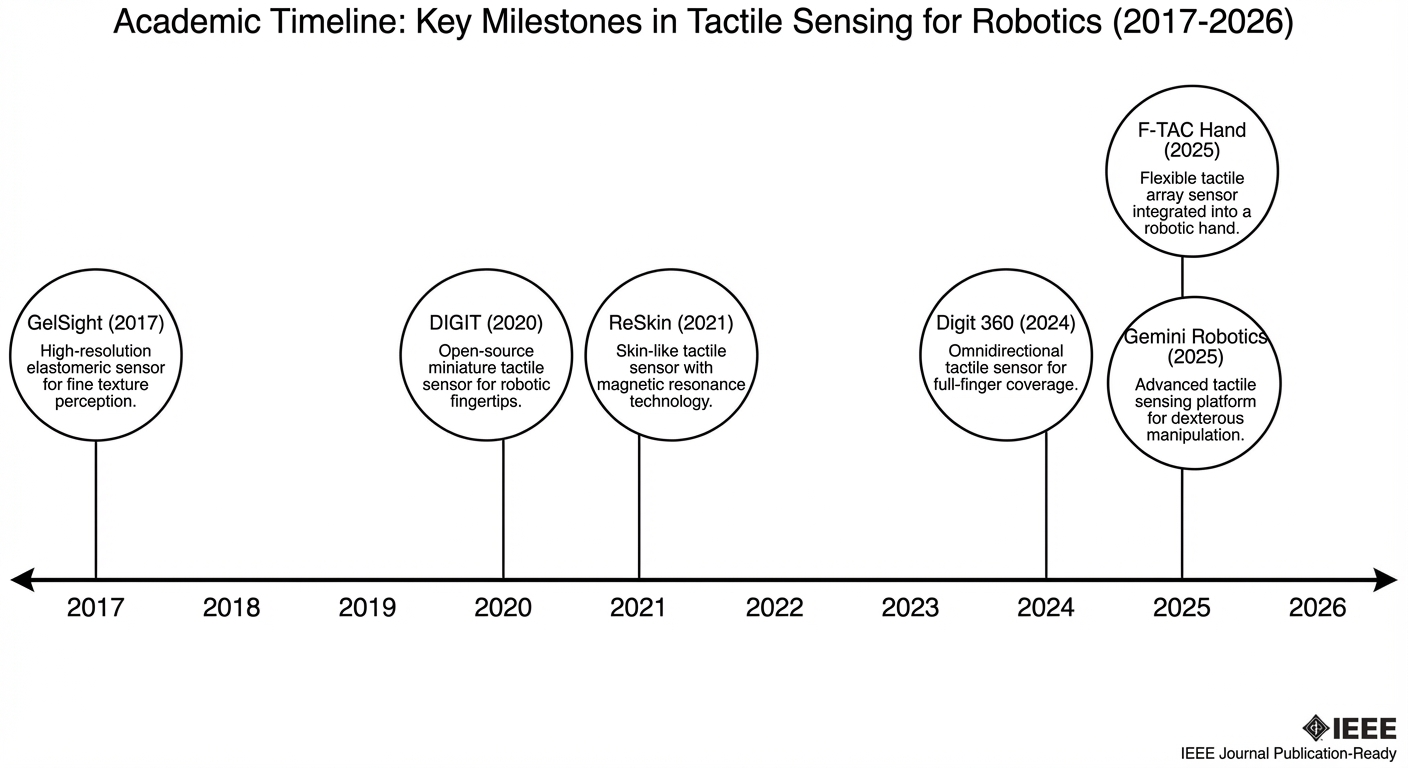
\includegraphics[width=\columnwidth]{../assets/figures/ch01/fig_1_2_timeline_academic.png}
\caption{Timeline of major milestones in tactile sensing for robot manipulation, from early transduction research through the GelSight revolution to modern VLA-based tactile integration.}
\label{fig:timeline}
\end{figure}

\subsection{Scope and Contributions}

This survey covers the full pipeline from tactile sensor hardware to learned dexterous manipulation policies, organized along six tightly coupled dimensions:
\begin{enumerate}
    \item \textbf{Tactile sensing technologies} (Section~\ref{sec:sensors}): five transduction principles, the GelSight--DIGIT--Digit~360 lineage, multi-axis sensing, and emerging neuromorphic/self-healing approaches.
    \item \textbf{Robot hand design and intelligent mechanisms} (Section~\ref{sec:hands}): the open-source ecosystem, actuation methods, and physical intelligence through underactuation, variable stiffness actuators, and active surfaces.
    \item \textbf{Data representation and collection} (Section~\ref{sec:data}): Albini et al.'s six-structure taxonomy~\cite{albini2025representing}, sensor-agnostic representations (AnyTouch~\cite{feng2025anytouch}, Canonical 3D~\cite{wu2025canonical}), public datasets, and tactile foundation models (Sparsh~\cite{higuera2024sparsh}, UniTouch~\cite{yang2024unitouch}).
    \item \textbf{Learning-based manipulation} (Section~\ref{sec:learning}): imitation learning (Diffusion Policy~\cite{chi2023diffusion}, ACT/ALOHA~\cite{zhao2023aloha}), reinforcement learning (DeXtreme~\cite{handa2023dextreme}), force-informed learning (DexForce~\cite{chen2025dexforce}, ForceVLA~\cite{yu2025forcevla}), and optimization alternatives.
    \item \textbf{VLA models} (Section~\ref{sec:vla}): from RT-1~\cite{brohan2023rt1} through pi0~\cite{black2024pi0} to Gemini Robotics~\cite{google2025gemini}, including tactile integration and post-deployment improvement via RECAP~\cite{pi2025recap}.
    \item \textbf{Human-to-robot transfer} (Section~\ref{sec:retarget}): kinematic retargeting (AnyTeleop~\cite{qin2023anyteleop}, ImMimic~\cite{liu2025immimic}), visual gap bridging (DexUMI~\cite{xu2025dexumi}), tactile gap solutions (OSMO~\cite{yin2025osmo}, UniTacHand~\cite{zhang2025unitachand}), and mechanical coupling (DEXOP~\cite{fang2025dexop}).
\end{enumerate}

We further analyze integrated systems and industrial applications (Section~\ref{sec:systems}), systematically identify the top~10 open challenges from 146 papers spanning 2020--2026 (Section~\ref{sec:discussion}), and propose the \emph{mechanism--tactile--learning triangle} as a unifying research direction for manufacturing-grade dexterous manipulation.

Our key contributions are:
\begin{itemize}
    \item The first survey to jointly cover tactile sensing hardware, dexterous hand design, VLA-based control, and embodiment retargeting within a single unified framework.
    \item A systematic identification and analysis of the top~10 open challenges based on frequency analysis across 146 recent papers.
    \item The mechanism--tactile--learning triangle: a proposed research direction that integrates physical intelligence (underactuation, VSA, active surfaces) with tactile perception and learned policies to reduce the burden on each individual axis.
\end{itemize}

\subsection{Comparison with Existing Surveys}

Several recent surveys address subsets of this space. The foundational review by Dahiya et al.~\cite{dahiya2010tactile} established the taxonomy of tactile transduction methods and remains the standard starting reference for the field. Albini et al.~\cite{albini2025representing} systematized tactile data representations into six canonical structures with selection guidelines based on hardware, task, and information requirements. Lepora~\cite{lepora2025past} traced four generations of tactile robotics history from the origins (1965--1979), through foundations and growth (1980--1994), the ``tactile winter'' (1995--2009), to the current expansion and diversification (2010--2024). The VLA systematic review~\cite{various2026vla} analyzed 102 models across 26 datasets and 12 simulation platforms, while ``What Matters in Building VLAs''~\cite{various2025whatmatters} (\emph{Nature Machine Intelligence}) found that hierarchical/late fusion architectures with diffusion decoders achieve the best generalization. A process-centric manipulation taxonomy~\cite{various2025taxonomy} (\emph{Nature Machine Intelligence}) formalized the connection from process specifications to tactile manipulation skills, validating 28 skills at near-100\% success rates.

However, \emph{no existing survey jointly covers tactile hardware, hand design, VLA-based control, and embodiment retargeting}. Sensor-focused surveys omit how sensing integrates with modern policy architectures; VLA surveys do not address the hardware and data collection dimensions; hand design reviews ignore the learning and transfer pipeline. This paper fills that gap by providing a unified treatment spanning the complete hardware--data--learning--transfer pipeline.

\subsection{Paper Organization}

The remainder of this paper is organized as follows. Section~\ref{sec:sensors} reviews tactile sensing technologies across five transduction principles. Section~\ref{sec:hands} covers robot hand design and intelligent mechanisms. Section~\ref{sec:data} addresses data representation, collection pipelines, and foundation models. Section~\ref{sec:learning} surveys learning-based manipulation including IL, RL, and force-informed approaches. Section~\ref{sec:vla} examines VLA models and their tactile integration. Section~\ref{sec:retarget} discusses embodiment retargeting. Section~\ref{sec:systems} presents integrated systems and industrial deployment. Section~\ref{sec:discussion} identifies open challenges and proposes the mechanism--tactile--learning triangle. Section~\ref{sec:conclusion} concludes.

\section{Tactile Sensing Technologies}
\label{sec:sensors}

This section reviews the principal transduction mechanisms, the dominant vision-based optical sensor paradigm, multi-axis sensing, sensor-integrated hand design, and emerging directions. The field has undergone a paradigm shift since 2017, driven by vision-based sensors that leverage the rich ecosystem of image processing and deep learning~\cite{dahiya2010tactile,lepora2025past}.

\begin{figure}[t]
\centering
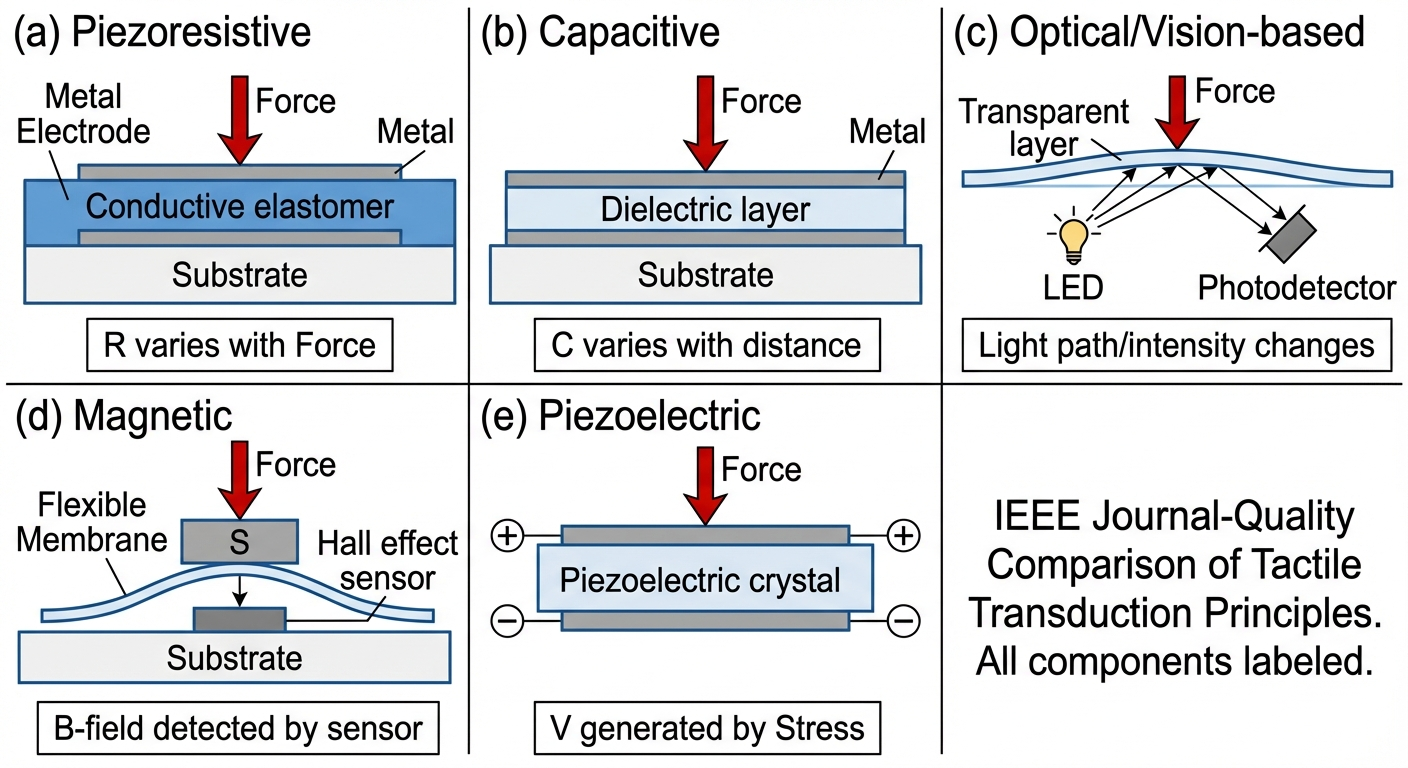
\includegraphics[width=\columnwidth]{../assets/figures/ch02/fig_2_1_transduction_principles_academic.png}
\caption{Taxonomy of tactile transduction principles. Five primary mechanisms---piezoresistive, capacitive, optical/vision-based, magnetic, and piezoelectric---each offer distinct trade-offs in resolution, durability, cost, and form factor.}
\label{fig:transduction_principles}
\end{figure}

\subsection{Transduction Principles}

Tactile sensors convert physical contact into electrical signals via five primary mechanisms, each with distinct trade-offs in resolution, durability, cost, and form factor~\cite{dahiya2010tactile}. Table~\ref{tab:sensors} provides a systematic comparison.

\textbf{Piezoresistive sensors} measure resistance change under pressure. Their simplicity and low cost make them the most widely deployed type. Sundaram et al.~\cite{sundaram2019stag} demonstrated the STAG glove with 548 piezoresistive sensors distributed across the human hand, capturing pressure signatures during natural grasping at high spatial resolution (\emph{Nature}, 2019). The resulting dataset enabled learning grasp-object associations from tactile patterns alone. Key limitations include hysteresis, temperature dependence, and drift under repeated loading, which necessitate periodic recalibration in long-duration applications.

\textbf{Capacitive sensors} detect changes in capacitance between electrode pairs separated by a deformable dielectric. A distinctive advantage is proximity sensing: the ability to detect approaching objects before physical contact occurs, providing pre-contact information unavailable to other sensor types. Murphy et al.~\cite{murphy2025capacitive} deployed 102 capacitive sensors for teaching by demonstration, demonstrating that the combination of pre-contact proximity and post-contact force data enhances policy learning. Susceptibility to electromagnetic interference and wiring complexity remain challenges for dense arrays.

\textbf{Magnetic sensors} combine permanent magnets with Hall-effect or magnetoresistive elements to measure deformation of a soft interface layer. ReSkin~\cite{bhirangi2021reskin} (Meta FAIR/CMU) introduced magnetic elastomer tactile skin at less than \$6 per unit, 2--3~mm thickness, and durability exceeding 50{,}000 interactions. The key innovation is separating the passive sensing surface from the electronics, enabling rapid replacement. AnySkin~\cite{bhirangi2024anyskin} advanced this to achieve \textbf{12-second plug-and-play replacement} without recalibration, maintaining 92\% slip detection accuracy across sensor instances. The OSMO glove~\cite{yin2025osmo} uses 12 three-axis magnetic sensors with MuMetal shielding for simultaneous normal and shear force measurement, serving as a cross-embodiment bridge between human and robot tactile data collection.

\textbf{Piezoelectric sensors} generate charge under dynamic deformation via materials such as PZT or PVDF. They excel at detecting vibration (40--400~Hz) and texture---functionally analogous to Pacinian corpuscles in biological touch~\cite{yu2025texture}. Their dynamic sensitivity makes them ideal for texture classification tasks, though they cannot measure static forces. Energy harvesting potential enables self-powered sensor designs.

\textbf{Optical/vision-based sensors} image the deformation of a transparent gel or elastomer using an embedded camera and reconstruct contact information from the resulting images. This approach has become the dominant paradigm since 2017 and is discussed in detail in the following subsection.

\begin{table*}[t]
\caption{Comparison of Tactile Sensor Technologies}
\label{tab:sensors}
\centering
\begin{tabular}{@{}lccccc@{}}
\toprule
\textbf{Property} & \textbf{Piezoresistive} & \textbf{Capacitive} & \textbf{Optical/Vision} & \textbf{Magnetic} & \textbf{Piezoelectric} \\
\midrule
Spatial resolution & Medium & Medium & Very high & Low--Medium & Low \\
Force range & Wide & Wide & Medium & Medium & Wide (dynamic) \\
Multi-axis sensing & Difficult & Possible & Excellent & Excellent & Difficult \\
Durability & Moderate & Moderate & Low (gel wear) & High & High \\
Cost per unit & Very low & Low & Medium (\$350) & Very low (\$6) & Medium \\
Form factor & Compact & Compact & Bulky (camera) & Compact & Compact \\
Proximity sensing & No & Yes & No & No & No \\
Representative & STAG~\cite{sundaram2019stag} & \cite{murphy2025capacitive} & DIGIT~\cite{lambeta2020digit} & ReSkin~\cite{bhirangi2021reskin} & --- \\
\bottomrule
\end{tabular}
\end{table*}

\begin{figure}[t]
\centering
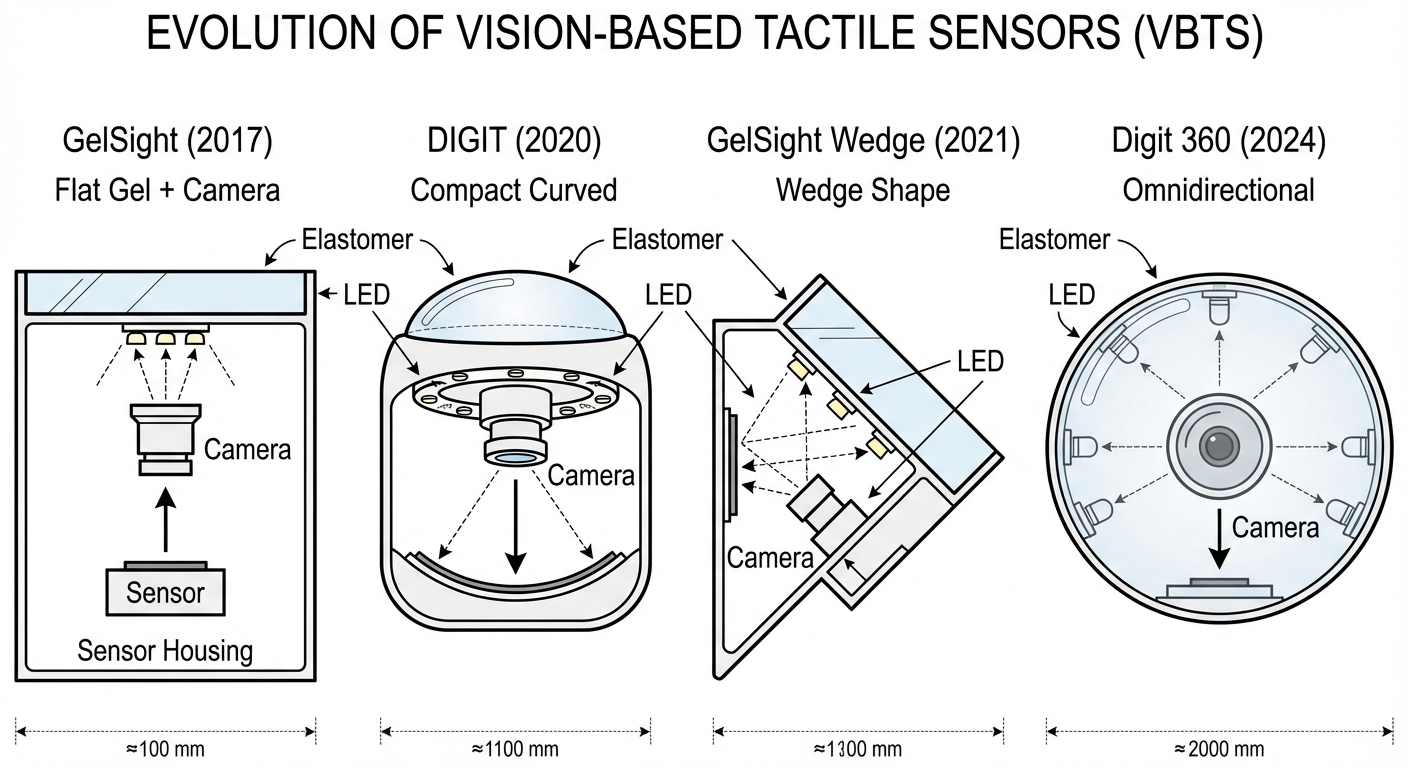
\includegraphics[width=\columnwidth]{../assets/figures/ch02/fig_2_2_vbts_evolution_academic.png}
\caption{Evolution of vision-based tactile sensors (VBTS): from GelSight (2017) through GelSight Wedge and DIGIT to Digit~360, showing progressive improvements in form factor, cost, resolution, and sensing modalities.}
\label{fig:vbts_evolution}
\end{figure}

\subsection{Vision-Based Optical Tactile Sensors}
\label{sec:vbts}

The introduction of GelSight~\cite{yuan2017gelsight} in 2017 marked a paradigm shift in tactile sensing. Using photometric stereo---multiple colored LEDs illuminate a coated elastomeric gel, and a camera captures the resulting shading patterns---GelSight reconstructs 3D contact surface geometry at micrometer resolution. This approach is paradigm-shifting because it imports the entire ecosystem of computer vision tools (CNNs, ViTs, self-supervised learning, diffusion models) to tactile perception, bypassing the need for specialized signal processing pipelines required by electrical transduction methods. With 600+ citations, GelSight established the vision-based tactile sensor (VBTS) family.

\textbf{GelSight Wedge}~\cite{wang2021wedge} (MIT CSAIL, ICRA 2021) redesigned the optical path into a wedge form factor compatible with standard parallel grippers, enabling integration into existing robotic systems rather than requiring custom hardware. This form factor innovation was critical for practical adoption.

\textbf{DIGIT}~\cite{lambeta2020digit} (Meta FAIR, 2020, 400+ citations) achieved the miniaturization and cost reduction needed for widespread adoption. At \$350---over 10$\times$ cheaper than BioTac (\$5K--10K)---and in a compact form factor suitable for mounting on individual fingers of multi-fingered hands, DIGIT became the de facto standard sensor for tactile manipulation research. Its open design catalyzed an ecosystem of downstream work in manipulation, representation learning, and sim-to-real transfer.

\textbf{Digit~360}~\cite{lambeta2024digit360} (Meta FAIR/GelSight, 2024) represents the most comprehensive artificial fingertip to date, integrating approximately 8.3 million taxels, 18+ sensing modalities (3D geometry, normal and shear force, vibration, temperature, proximity), omnidirectional surface coverage, and 1~mN force resolution approaching human sensitivity (3~mN for Meissner corpuscles). Digit~360 integrates multimodal sensing corresponding to multiple human receptor types into a single fingertip, representing the closest attempt yet to a ``complete'' artificial touch organ.

\textbf{Modular design}~\cite{agarwal2025modular} (CMU, \emph{IJRR} 2025) proposed a systematic framework for GelSight-family sensors, enabling customization by modularly combining gel materials, illumination layouts, camera positions, and housings to match application requirements.

The primary limitation of VBTS remains \textbf{durability}. Gel surfaces wear with repeated contact; light sources degrade; dust infiltration and cleaning difficulty constrain long-term industrial operation. When the F-TAC Hand~\cite{zhao2025ftac} placed 17 sensors across the hand, it also introduced 17 potential failure points. AnySkin's 12-second replacement approach~\cite{bhirangi2024anyskin} offers one practical mitigation strategy (see Section~\ref{sec:discussion}).

\subsection{Multi-Axis Sensing}

Normal force alone is insufficient for robust manipulation. Shear (tangential) forces provide critical information for three capabilities: (1)~\textbf{slip detection}---shear force changes are leading indicators of incipient slip, enabling preemptive grip force increase before the object actually slides~\cite{zhao2025slip}; (2)~\textbf{object orientation estimation}---tangential force vectors reveal object tilt relative to the gripper~\cite{hossain2025multiaxis}; and (3)~\textbf{force-noise decoupling}---multi-axis information separates true contact forces from sensor noise and external vibration~\cite{cho2025decoupling}. Multi-dimensional tactile data has also been shown to improve policy sample efficiency in learning-based manipulation.

The OSMO glove~\cite{yin2025osmo} exemplifies practical multi-axis design: 12 three-axis magnetic sensors with MuMetal shielding measure simultaneous normal and shear forces across fingertips and palm. Its open-source design and ``embodiment bridge'' concept---using the same glove on both human and robot to eliminate the tactile domain gap---represent an emerging paradigm for cross-embodiment data collection (see Section~\ref{sec:retarget}).

\subsection{Sensor-Integrated Hand Design}

Sensor technology achieves maximum impact when co-optimized with hand design rather than retrofitted. The F-TAC Hand~\cite{zhao2025ftac} (\emph{Nature Machine Intelligence}, 2025) demonstrated this principle: 17 vision-based tactile sensors were placed based on optimized contact probability distributions, covering 70\% of the hand surface at 0.1~mm resolution. The result was 100\% multi-object grasp success---a direct demonstration that integrated tactile feedback transforms manipulation performance. 3D-ViTac~\cite{huang2024vitac} (CoRL 2024) fused dense tactile sensors (3~mm$^2$ resolution) with vision into a unified 3D representation, achieving 85--90\% success on bimanual dexterous tasks versus 45--50\% with vision only.

\subsection{Emerging Directions}

\textbf{Neuromorphic tactile sensors} mimic the biological nervous system's event-driven processing to maximize energy efficiency and temporal resolution. NRE-skin~\cite{gao2025nreskin} (\emph{PNAS}, 2025) implements a hierarchical neural-inspired architecture enabling high-resolution touch sensing, active pain/injury detection with local reflexes, and modular quick-release repair. Spike-based encoding achieves 10$\times$ super-resolution through CMOS/memristor hardware combined with spiking neural network (SNN) decoding~\cite{various2025spike}. Bioinspired spiking architectures have demonstrated efficient tactile encoding under energy constraints (\emph{Nature Communications}, 2026).

\textbf{Self-healing electronic skin} addresses durability through materials science. Multisensory e-skin with decoupled pressure-temperature sensing and self-healing properties~\cite{various2025eskin} has the potential to fundamentally resolve the sensor durability challenge in industrial environments.

\textbf{Physically-based rendering (PBR) for sensor design}~\cite{various2025pbr} (\emph{Nature Communications Engineering}, 2025) enables simulation-driven design of optical tactile sensors, reducing fabrication trial-and-error and supporting digital twin-based development workflows.

\section{Robot Hand Design and Intelligent Mechanisms}
\label{sec:hands}

The mechanical platform determines what a tactile sensing system can achieve. This section reviews the design spectrum from parallel grippers to multi-fingered hands, the open-source revolution that democratized dexterous manipulation research, actuation methods, and three classes of intelligent mechanisms that embed physical intelligence into the gripper structure.

\subsection{Design Spectrum: Grippers to Dexterous Hands}

Robot end-effectors span a continuum from simple parallel grippers (2 fingers, 1 DoF) to fully anthropomorphic hands (5 fingers, 20+ DoF). Parallel grippers dominate industrial deployment due to their simplicity and reliability, but suffer from poor shape adaptation, inability to maintain continuous contact, and vulnerability with thin or multiple objects. Dexterous hands offer diverse grasp types and in-hand manipulation but introduce control complexity, combinatorial explosion of contact states, high cost, and frequent hardware failures~\cite{bicchi2000simplicity,bicchi2000grasping}.

Bicchi's landmark argument for simplicity~\cite{bicchi2000simplicity} resolved this tension by introducing \emph{underactuation} (fewer actuators than joints) and \emph{synergy} (coordinated multi-joint patterns), demonstrating that most everyday grasps can be explained by 2--3 principal synergies extracted via PCA. This insight directly shaped modern affordable hands including the SoftHand family and LEAP Hand.

\begin{figure}[t]
\centering
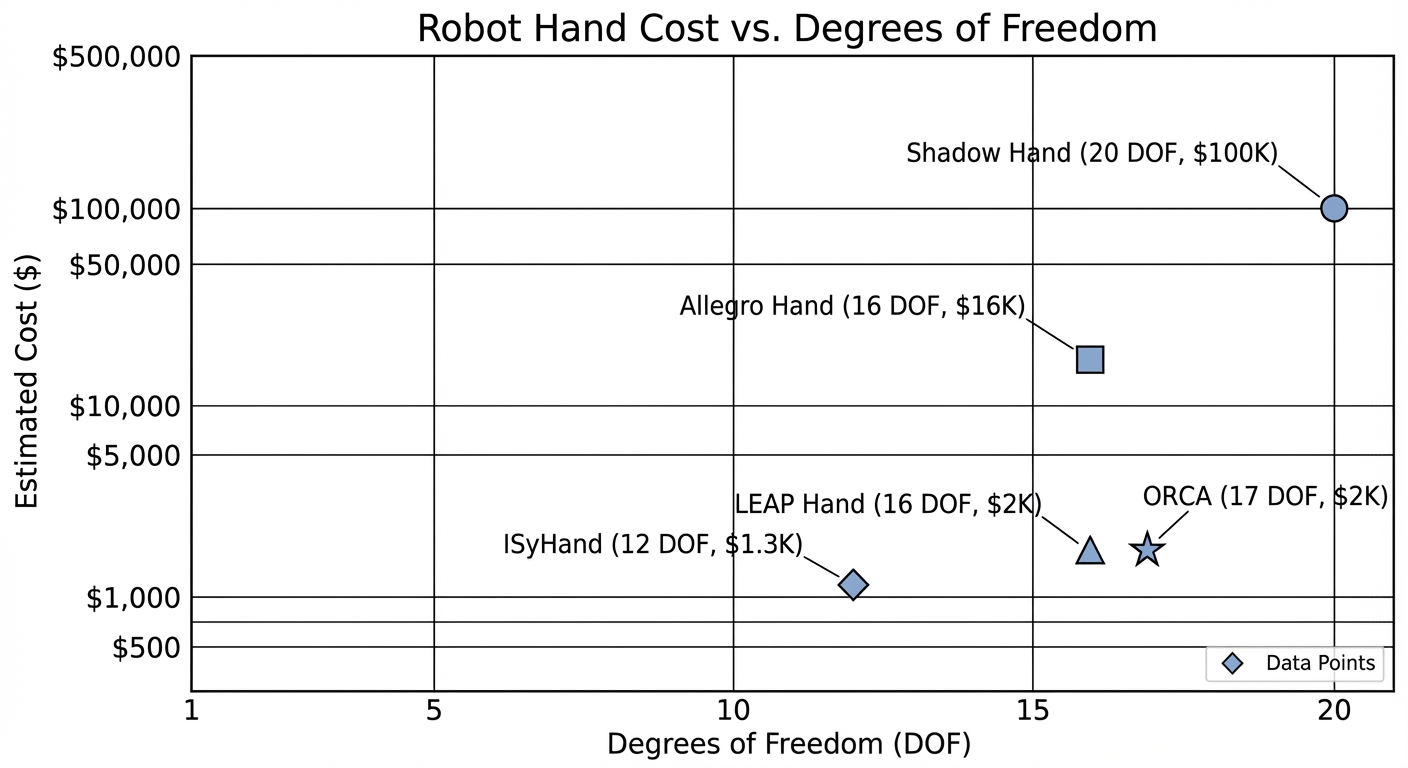
\includegraphics[width=\columnwidth]{../assets/figures/ch04/fig_4_2_hand_cost_performance_academic.png}
\caption{Cost--performance landscape of dexterous robot hands. The open-source revolution (2023--2025) reduced entry costs by 50$\times$, from Shadow Hand (\$100K+) to LEAP Hand (\$2K) and ISyHand (\$1.3K), while maintaining or improving manipulation performance.}
\label{fig:hand_cost_performance}
\end{figure}

\subsection{The Open-Source Revolution}

Since 2023, low-cost open-source dexterous hands have fundamentally transformed the research ecosystem by reducing the entry cost by 50$\times$. Table~\ref{tab:hands} compares the major platforms.

\begin{table*}[t]
\caption{Comparison of Dexterous Robot Hands}
\label{tab:hands}
\centering
\begin{tabular}{@{}lcccccc@{}}
\toprule
\textbf{Hand} & \textbf{Cost} & \textbf{DoF} & \textbf{Actuation} & \textbf{Tactile} & \textbf{Open-Source} & \textbf{Year} \\
\midrule
Shadow Hand & \$100K+ & 24 & Tendon/pneumatic & BioTac (opt.) & No & 1990s \\
Allegro Hand & \$16K & 16 & Direct drive & No & No & 2012 \\
LEAP Hand~\cite{shaw2023leap} & \$2K & 16 & Direct drive & No & Yes & 2023 \\
ISyHand~\cite{richardson2025isyhand} & \$1.3K & var. & Direct drive & No & Yes & 2025 \\
ORCA~\cite{christoph2025orca} & \$2K & 17 & Tendon & Yes & Yes & 2025 \\
F-TAC Hand~\cite{zhao2025ftac} & --- & var. & var. & 17 sensors & Partial & 2025 \\
\bottomrule
\end{tabular}
\end{table*}

\textbf{LEAP Hand}~\cite{shaw2023leap} (CMU, RSS 2023, 200+ citations) established the open-source paradigm: a 3D-printable, 4-finger, 16-DoF hand costing \$2K that outperforms the \$16K Allegro Hand on benchmark tasks. Its novel kinematic structure reproduces the essential degrees of freedom of the human hand using only low-cost servo motors and 3D-printed components. The design philosophy---``maximum dexterity at minimum cost''---catalyzed a wave of follow-on work.

\textbf{ISyHand}~\cite{richardson2025isyhand} (MPI, IEEE Humanoids 2025) further reduced cost to \$1.3K while introducing an \emph{articulated palm} that increases overall dexterity with modest sacrifice in anthropomorphism. Assembly requires only 4 hours from off-the-shelf Dynamixel motors and 3D-printed parts.

\textbf{ORCA}~\cite{christoph2025orca} (ETH Zurich) provides a 17-DoF tendon-driven hand with \emph{integrated tactile sensors}, built for under 2{,}000~CHF in 8 hours. Key reliability features---popping joints, auto-calibration, and tensioning systems---reduce maintenance complexity, enabling continuous learning without frequent hardware intervention. The commercial spinoff Mimic Robotics is pursuing factory-grade deployment.

The \textbf{F-TAC Hand}~\cite{zhao2025ftac} (\emph{Nature Machine Intelligence}, 2025) demonstrated the value of sensor-integrated co-design: 17 vision-based tactile sensors placed according to contact probability distributions cover 70\% of the hand surface at 0.1~mm resolution, achieving 100\% multi-object grasp success---a metric that no non-tactile hand has matched.

The Allegro Hand (\$16K, Wonik Robotics) served as the de facto research standard prior to the open-source wave and remains prominent in sim-to-real work including DeXtreme~\cite{handa2023dextreme} and the RGMC competition~\cite{yu2025rgmc}. Wonik's ongoing Digit Plexus integration with Meta FAIR represents a step toward standardized sensor-hand interfaces.

\subsection{Actuation Methods}

Four actuation methods dominate, each with distinct trade-offs:

\textbf{Direct drive} couples motors directly to joints (Allegro, LEAP). Advantages: fast control response, simple kinematics, precise position control. Disadvantage: motor size constrains finger miniaturization.

\textbf{Tendon-driven} designs place actuators remotely and transmit force via tendons (SoftHand~\cite{catalano2014softhand}, ORCA~\cite{christoph2025orca}, Shadow Hand). Advantages: finger miniaturization, natural compliance, reduced distal mass. Disadvantage: tendon routing complexity, friction losses, wear.

\textbf{Hydraulic} actuation (Sanctuary AI Phoenix Gen~8) achieves high power density with 20~DoF and 5~mN tactile sensitivity---the most advanced tactile integration among commercial humanoids. The 50$\times$ faster, 6$\times$ cheaper miniaturized valves represent a significant engineering achievement. Disadvantage: system complexity and cost.

\textbf{Pneumatic} actuation using McKibben muscles~\cite{alabeach2017vsa} provides inherent compliance and variable stiffness through antagonistic arrangements. Well suited for safe human-proximity operation but offers lower control precision than electric alternatives.

\subsection{Intelligent Mechanisms}
\label{sec:mechanisms}

Three classes of mechanisms embed ``physical intelligence'' into gripper design, reducing the burden on sensing and learning systems.

\subsubsection{Underactuation}

Underactuated hands use fewer actuators than joints, with remaining joints determined passively by springs or mechanical stops. The core value is \emph{automatic shape adaptation}: the mechanism itself, not a control algorithm, conforms to object geometry.

The Pisa/IIT SoftHand family exemplifies this approach. SoftHand~1~\cite{catalano2014softhand} (\emph{IJRR}, 2014, 500+ citations) drives 19 joints with a single actuator via adaptive synergy---all joints coordinate along the first principal synergy, and tendons slip on contact to automatically expand the contact area. SoftHand~2~\cite{dellasantina2018softhand2} (\emph{IEEE T-RO}, 2018) added a second actuator with friction-based actuation expansion for more diverse grasp types. Capsi-Morales et al.~\cite{capsimorales2020palm} extended adaptability to the palm itself by sectioning and connecting palm segments via underactuation.

\subsubsection{Variable Stiffness Actuators (VSA)}

VSAs enable a single mechanism to transition between compliant and stiff states, addressing the fundamental tension between compliance (needed for safe contact) and rigidity (needed for stable grasping). Four implementation approaches have been demonstrated: (1)~parallel beam with slider-adjustable effective length, achieving 70.9$\times$ stiffness ratio with ArUco marker-based vision force sensing~\cite{fu2023vsa}; (2)~McKibben muscle antagonistic arrangement enabling independent pose-stiffness control with 150\%+ stiffness increase~\cite{alabeach2017vsa}; (3)~SMA actuation combined with SMP stiffness switching, achieving 55$\times$ change per hinge~\cite{wang2017sma}; and (4)~particle jamming with fiber-reinforced pneumatic actuators for 10$\times$+ stiffness enhancement~\cite{wei2016jamming}.

\subsubsection{Active Surfaces}

Active surfaces drive the gripper's contact surface itself---typically via belts or rollers---enabling manipulation while maintaining contact. This addresses thin-object approach (pulling cards from a table), in-grasp repositioning (adjusting object position without releasing), and continuous-contact manipulation~\cite{kim2024lbh,wang2025belt}. The key insight is that \emph{continuous contact is easier to control and more stable than discrete release-and-regrasp}, because it eliminates the uncertainty of contact state transitions.

\subsubsection{Temporal Integration}

The most powerful approach combines all three mechanisms in temporal sequence: (1)~underactuation for initial shape adaptation during approach, (2)~VSA for stiffness transition to lock the grasp, and (3)~active surfaces for in-grasp manipulation and repositioning. This sequence mirrors the natural human grasping flow---approach, grasp, adjust---through purely mechanical means. The synergy of these three mechanisms creates capabilities beyond the sum of their individual contributions, particularly for factory automation scenarios involving thin objects, multiple objects, and precision repositioning. This physical intelligence concept forms one axis of the mechanism--tactile--learning triangle proposed in Section~\ref{sec:discussion}.

\section{Tactile Data Representation and Collection}
\label{sec:data}

If tactile sensors convert contact into signals, the question of how to \emph{structure} those signals, how to \emph{collect} them at scale, and how to build \emph{general-purpose representations} through pretraining defines the data foundation for learned manipulation. This section reviews the representation taxonomy, sensor-agnostic approaches, public datasets, foundation models, and collection pipelines.

\begin{figure}[t]
\centering
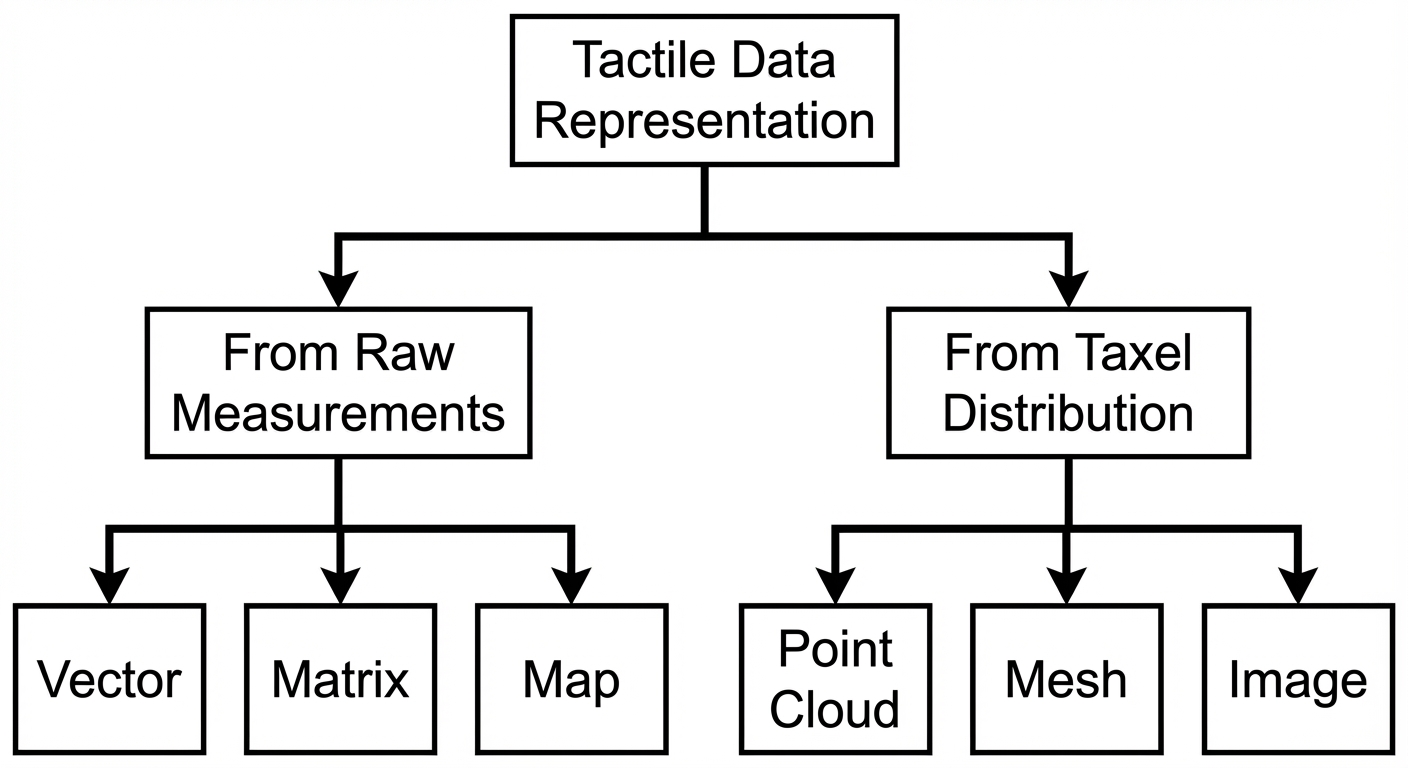
\includegraphics[width=\columnwidth]{../assets/figures/ch03/fig_3_1_albini_taxonomy_academic.png}
\caption{Albini et al.'s six-structure taxonomy of tactile data representations: vector, matrix, map, point cloud, mesh, and image. Selection depends on sensor hardware, task requirements, and information needs.}
\label{fig:albini_taxonomy}
\end{figure}

\subsection{Representation Taxonomy}

Albini et al.~\cite{albini2025representing} (submitted to \emph{IEEE T-RO}) systematized tactile data representations into six canonical structures, providing selection guidelines based on hardware output characteristics, task requirements, and information needs:

\begin{enumerate}
    \item \textbf{Vector}: The simplest form---each sensor's readings arranged as a 1D vector (e.g., OSMO's 36-dimensional force vector from 12 three-axis sensors~\cite{yin2025osmo}). Suitable for classification, force control, and slip detection, but loses spatial relationship information.
    \item \textbf{Matrix}: Sensor array outputs as a 2D grid (e.g., STAG's 548-sensor pressure matrix~\cite{sundaram2019stag}). Natural for contact pattern classification but distorted when sensors are placed on curved surfaces.
    \item \textbf{Map}: Data projected onto a reference surface. UniTacHand~\cite{zhang2025unitachand} projects both human glove and robot tactile data onto MANO UV maps, creating a shared representation space for cross-embodiment transfer (see Section~\ref{sec:retarget}).
    \item \textbf{Point cloud}: Contact points with 3D coordinates. Robot Synesthesia~\cite{yuan2024synesthesia} (ICRA 2024) used PointNet to process tactile point clouds for visuotactile in-hand manipulation, achieving generalization to novel objects including double-ball rotation and 3-axis reorientation.
    \item \textbf{Mesh}: Triangulated contact surfaces for FEM-based deformation simulation. DiffTactile~\cite{si2024difftactile} (ICLR 2024) uses mesh-based contact modeling in a differentiable simulator supporting gradient-based optimization.
    \item \textbf{Image}: The raw output of vision-based tactile sensors is already an image, enabling direct application of CNNs, ViTs, and the full vision model ecosystem. Currently the most widely used representation due to the dominance of GelSight/DIGIT sensors.
\end{enumerate}

The choice of representation directly impacts learning performance. Wu et al.~\cite{wu2025canonical} (ICRA 2025) demonstrated that transforming raw sensor output into a \emph{canonical 3D coordinate frame} enables task-agnostic transfer: a two-stage pipeline of play-data pretraining followed by few-shot expert fine-tuning achieved 78\% average success versus 63\% for T-DEX, representing a 24\% relative improvement from the representation choice alone.

\subsection{Sensor-Agnostic Representations}

A fundamental limitation is \emph{sensor specificity}: representations learned on GelSight do not transfer to DIGIT, and DIGIT representations fail on ReSkin. Three approaches address this challenge, each targeting the ``CLIP moment'' for touch---aligning diverse sensor outputs into a unified embedding space:

\textbf{AnyTouch}~\cite{feng2025anytouch} (ICLR 2025) learns unified static-dynamic representations across multiple vision-based tactile sensors through a multi-level framework, introducing the TacQuad aligned multi-modal multi-sensor dataset.

\textbf{Sensor-Invariant Representation}~\cite{various2025sensorinvariant} achieves zero-shot transfer across optical sensor designs by stripping sensor-specific information while preserving essential contact characteristics.

\textbf{Canonical 3D Tactile}~\cite{wu2025canonical} transforms raw sensor output into a 3D canonical coordinate frame, constructing sensor-independent representations that combine with task-agnostic play data pretraining for efficient transfer.

\subsection{Public Datasets}

The scale of tactile datasets remains orders of magnitude smaller than vision datasets, representing a fundamental bottleneck for foundation model development. Table~\ref{tab:datasets} summarizes major public datasets.

\begin{table}[t]
\caption{Major Tactile Datasets}
\label{tab:datasets}
\centering
\begin{tabular}{@{}L{2.2cm}L{1.8cm}cc@{}}
\toprule
\textbf{Dataset} & \textbf{Scale} & \textbf{Modal.} & \textbf{Year} \\
\midrule
Touch-and-Go~\cite{yang2022touchandgo} & 3M+ contacts & V+T & 2023 \\
Touch100k~\cite{yang2024touch100k} & 100K+ images & T & 2024 \\
VTDexManip~\cite{liu2025vtdexmanip} & 10 tasks, 182 obj. & V+T & 2025 \\
OXE~\cite{oxe2024} & 1M+ traj., 22 emb. & V+A & 2024 \\
\bottomrule
\end{tabular}
\end{table}

VTDexManip~\cite{liu2025vtdexmanip} (ICLR 2025) is a significant milestone---the first large-scale visual-tactile dataset from actual human demonstrations of dexterous manipulation, spanning 10 tasks and 182 objects with an RL benchmark. Open X-Embodiment~\cite{oxe2024} (ICRA 2024) is the largest robot manipulation dataset (1M+ trajectories from 22 embodiments, 34 labs) but includes tactile data in only a small subset. Expanding from Touch-and-Go's 3M contacts to the 100M+ scale needed for robust foundation models remains a key open challenge.

\subsection{Tactile Foundation Models}

Two approaches pursue the ``ImageNet moment'' for touch through self-supervised pretraining:

\textbf{Sparsh}~\cite{higuera2024sparsh} (Meta FAIR/CMU/Berkeley, CoRL 2024) is a self-supervised tactile foundation model pretrained on 460K+ images from multiple vision-based tactile sensors. Its significance lies in being the first large-scale attempt to replicate for touch what ImageNet pretraining accomplished for vision. However, 460K images remain two orders of magnitude below ImageNet's 14M, and a 10$\times$+ expansion is needed for robust generalization.

\textbf{UniTouch}~\cite{yang2024unitouch} (CVPR 2024) uses contrastive learning to align touch with vision, language, and audio into a unified embedding space---analogous to CLIP for vision-language. This enables zero-shot tactile classification and cross-modal retrieval without task-specific fine-tuning, demonstrating that the semantic structure of touch can be captured through alignment with other modalities.

\subsection{Data Collection Pipelines}

Collecting tactile data is inherently harder than visual data because physical contact is required. Four approaches span the throughput-quality trade-off:

\textbf{Teleoperation} yields the highest-quality demonstrations but at $\sim$10 demos/hr throughput. AnyTeleop~\cite{qin2023anyteleop} (RSS 2023) provides general-purpose vision-based dexterous teleoperation via Dex-Retarget. Bunny-VisionPro~\cite{ding2024bunny} achieves research-grade teleoperation using consumer Apple Vision Pro hardware.

\textbf{Portable motion capture}: DexCap~\cite{wang2024dexcap} (Stanford, RSS 2024) achieves 3$\times$ faster data collection than standard teleoperation, with policy learning from just 30 minutes of data.

\textbf{Kinesthetic teaching}: DexForce~\cite{chen2025dexforce} (\emph{IEEE RA-L}) uses a spring model ($x_f = x_o + k_f \cdot f$, single parameter $k_f = 0.0045$) to naturally record force-torque information during physical guidance, capturing richer contact dynamics than teleoperation.

\textbf{Synthetic data}: NVIDIA's Isaac Sim pipeline generates 780K trajectories (equivalent to 6{,}500 hours of real data) in just 11 hours, improving real-world performance by 40\%~\cite{nvidia2025synthetic}. Open-source simulators Tacto~\cite{wang2022tacto} (PyRender + PyBullet for vision-based sensors) and DiffTactile~\cite{si2024difftactile} (differentiable FEM-based contact) enable sim-to-real tactile training.

\section{Learning-Based Tactile Manipulation}
\label{sec:learning}

This section surveys three paradigms for learning manipulation with tactile feedback---imitation learning, reinforcement learning, and force-informed approaches---along with optimization-based alternatives that compete with learned policies on structured tasks. Table~\ref{tab:learning} provides a comparative overview.

\begin{figure}[t]
\centering
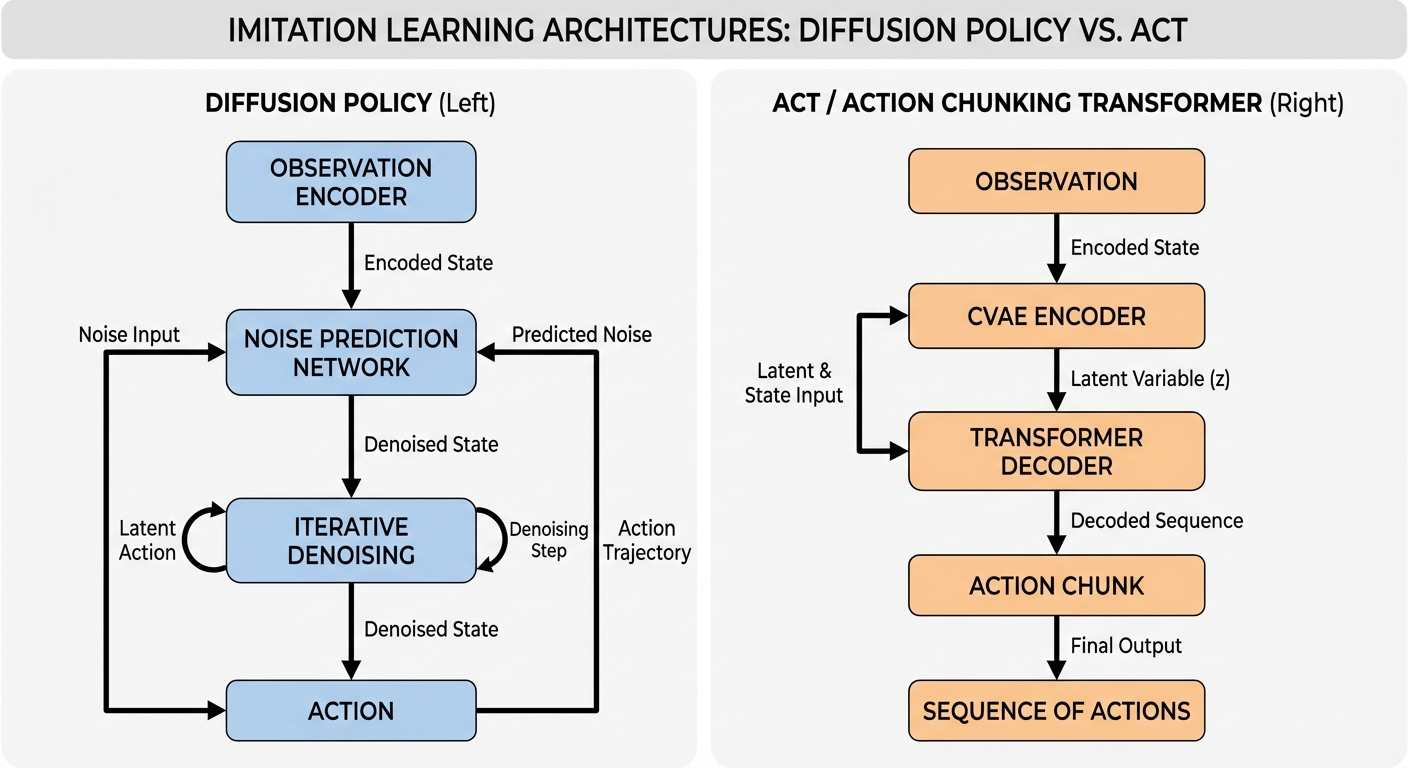
\includegraphics[width=\columnwidth]{../assets/figures/ch07/fig_7_1_diffusion_vs_act_academic.png}
\caption{Comparison of the two dominant imitation learning architectures for tactile manipulation: Diffusion Policy (conditional denoising process) and ACT/ALOHA (action chunking with Transformers). Both handle multimodal action distributions but differ in generation mechanism and temporal structure.}
\label{fig:il_architectures}
\end{figure}

\subsection{Imitation Learning}

Imitation learning (IL) trains policies by directly mimicking human demonstrations. Two architectures have dominated since 2023, both leveraging the expressivity of generative models to handle the multimodal action distributions characteristic of contact-rich manipulation.

\textbf{Diffusion Policy}~\cite{chi2023diffusion} (Columbia/MIT/TRI, RSS 2023, 500+ citations) models the robot's visuomotor policy as a conditional denoising diffusion process. Starting from Gaussian noise, iterative denoising produces action sequences conditioned on the current observation. This formulation naturally handles multimodal action distributions---a critical requirement when multiple valid manipulation strategies exist for the same observation---achieving 46.9\% average improvement over prior deterministic and VAE-based methods. The architecture's compatibility with tactile conditioning has made it the preferred backbone for contact-rich tasks: FARM~\cite{helmut2025farm} conditions Diffusion Policy on GelSight Mini tactile images for force-aware manipulation, while PP-Tac~\cite{lin2025pptac} integrates slip detection with diffusion-based control for thin-object grasping.

\textbf{ACT/ALOHA}~\cite{zhao2023aloha} (Stanford, RSS 2023, 400+ citations) takes a different approach via Action Chunking with Transformers (ACT), predicting sequences of future actions rather than single-step outputs. The key insight is that temporal chunking reduces the compounding error problem in sequential decision-making. On the sub-\$20K ALOHA bimanual hardware, ACT achieves 80--90\% success on fine-grained bimanual tasks from just 10-minute demonstrations---a data efficiency that makes the approach practical for rapid prototyping. Mobile ALOHA~\cite{fu2024mobilealoha} (200+ citations) extends the platform to mobile bimanual manipulation, representing one of the most influential end-to-end research systems.

\begin{figure}[t]
\centering
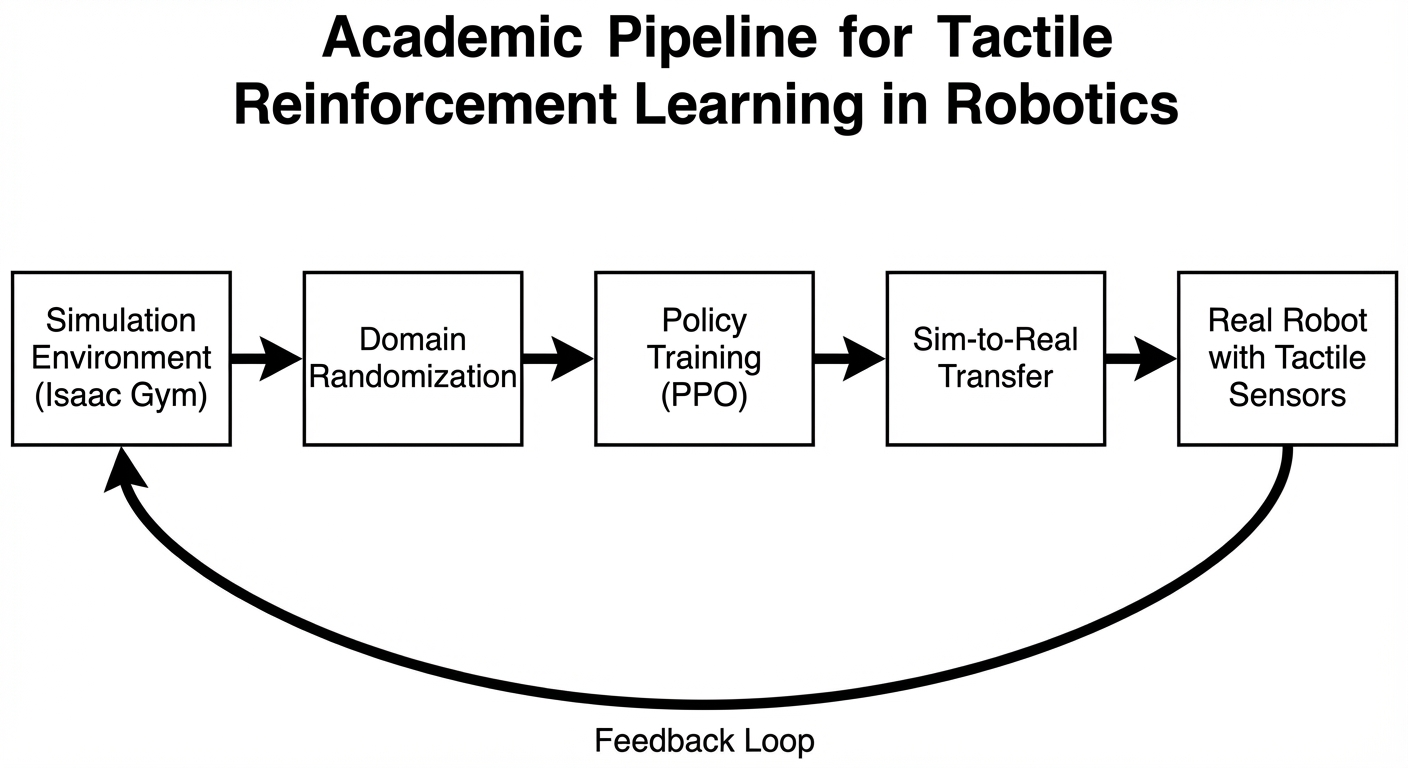
\includegraphics[width=\columnwidth]{../assets/figures/ch07/fig_7_2_tactile_rl_pipeline_academic.png}
\caption{Tactile reinforcement learning pipeline: policies are trained in simulation with domain randomization (physics and tactile parameters) and transferred zero-shot to real hardware. Binary tactile skin models with wide coverage have proven surprisingly effective for sim-to-real transfer.}
\label{fig:tactile_rl_pipeline}
\end{figure}

\subsection{Reinforcement Learning}

Reinforcement learning (RL) discovers manipulation policies through trial-and-error optimization of a reward signal, typically in simulation with subsequent transfer to physical hardware.

\textbf{OpenAI Dactyl}~\cite{openai2020dactyl} (\emph{IJRR}, 2020, 1{,}500+ citations) was the landmark demonstration that sim-to-real RL can solve contact-rich dexterous manipulation. Using a Shadow Hand in simulation with massive domain randomization, Dactyl learned to manipulate a Rubik's Cube and transferred zero-shot to the physical robot. The work established domain randomization as the primary strategy for overcoming the sim-to-real gap.

\textbf{DeXtreme}~\cite{handa2023dextreme} (NVIDIA, ICRA 2023, 200+ citations) advanced the state of the art with Automatic Domain Randomization (ADR) on Allegro Hand in Isaac Gym. ADR simultaneously randomizes both physics parameters (friction, mass, joint stiffness, gravity) and non-physics parameters (lighting, camera position, texture, background), with the randomization ranges automatically adjusted based on training progress. Combined with Omniverse Replicator for synthetic visual data, vision-based policies outperformed all prior literature on dexterous manipulation benchmarks.

\textbf{Tactile RL} has demonstrated that simplified sensor models with wide coverage can be surprisingly effective. Yin et al.~\cite{yin2023rotating} (RSS 2023) achieved continuous in-hand rotation using only binary tactile sensors---contact yes/no plus 3-axis direction---without any vision. The subsequent work~\cite{yin2024tactile} developed a binary 3-axis tactile skin simulation model running at 5{,}000~FPS, enabling zero-shot sim-to-real transfer with 93\% success on out-of-distribution objects. This result challenges the assumption that high-resolution sensors are always better: \emph{coverage of the entire hand surface may matter more than resolution at any single point}.

Human-in-the-loop RL~\cite{luo2025hil} (\emph{Science Robotics}, 2025) combines human intuition with autonomous policy optimization, achieving near-perfect success rates on precise assembly tasks within 1--2.5 hours of real-world training, outperforming pure RL baselines by 2$\times$.

\subsection{Tactile-Based Manipulation Methods}

\begin{table*}[t]
\caption{Comparison of Learning Methods for Tactile Manipulation}
\label{tab:learning}
\centering
\begin{tabular}{@{}L{2.8cm}cL{2.8cm}L{2.5cm}c@{}}
\toprule
\textbf{Method} & \textbf{Year} & \textbf{Approach} & \textbf{Tactile Input} & \textbf{Key Result} \\
\midrule
Yin et al.~\cite{yin2023rotating} & 2023 & RL, binary tactile & Binary 3-axis skin & 93\% OOD \\
Wu et al.~\cite{wu2025canonical} & 2025 & IL, canonical 3D & 3-axis tactile & 78\% avg \\
PP-Tac~\cite{lin2025pptac} & 2025 & Diffusion + slip & R-Tac sensor & 87.5\% thin \\
DexForce~\cite{chen2025dexforce} & 2025 & IL, spring model & 6-axis F/T & 76\% avg \\
ForceVLA~\cite{yu2025forcevla} & 2025 & VLA + MoE & 6-axis F/T & +23.2pp \\
FARM~\cite{helmut2025farm} & 2026 & Diffusion + tactile & GelSight Mini & Force-aware \\
TLA~\cite{hao2025tla} & 2025 & Language + tactile & 24K pairs & 85+\% \\
RGMC~\cite{yu2025rgmc} & 2025 & Optimization & Kinematic only & 5mm error \\
\bottomrule
\end{tabular}
\end{table*}

Several recent works demonstrate tactile feedback as increasingly critical for specific manipulation capabilities:

\textbf{PP-Tac}~\cite{lin2025pptac} (RSS 2025) addresses the extremely challenging problem of grasping thin objects---paper, cards, gaskets---where standard grippers fail completely. The system integrates an R-Tac round camera-based gel sensor, a lightweight CNN for real-time slip detection, an online force controller, and Diffusion Policy into a unified pipeline, achieving 87.5\% success on thin and deformable objects. This result demonstrates tactile's direct practical value on problems that vision alone cannot solve.

\textbf{TLA}~\cite{hao2025tla} (Tactile-Language-Action model) processes sequential tactile feedback via cross-modal language grounding, enabling natural language commands for contact-rich manipulation. With 24{,}000 tactile-action instruction pairs customized for fingertip peg-in-hole assembly, TLA achieves 85+\% success on unseen clearances and peg shapes, significantly outperforming standard diffusion policy baselines.

\subsection{Force-Informed Learning}

Two approaches explicitly integrate force information as a first-class modality:

\textbf{DexForce}~\cite{chen2025dexforce} (\emph{IEEE RA-L}) addresses the force information gap in teleoperation-collected demonstrations. Using a spring model $x_f = x_o + k_f \cdot f$ with a single parameter $k_f = 0.0045$, kinesthetic teaching naturally records force-torque information that teleoperation misses. Policies trained on force-informed actions achieve 76\% average success across 6 contact-rich tasks, while policies trained without force information achieve near-zero success---a dramatic demonstration that force is essential, not optional, for these tasks.

\textbf{ForceVLA}~\cite{yu2025forcevla} (NeurIPS 2025) introduces FVLMoE, a 4-expert Mixture-of-Experts architecture that dynamically routes force, vision, and language inputs based on task demands within a pi0-based VLA framework. The result is +23.2 percentage points over force-free baselines and 90\% success under visual occlusion---conditions where vision-only policies fail catastrophically. ForceVLA represents the direction of integrating tactile/force as a ``first-class modality'' in foundation models for manipulation.

\subsection{Optimization-Based Alternatives}

Not all manipulation requires learning. The RGMC Champion solution~\cite{yu2025rgmc} (\emph{IEEE RA-L}, ICRA 2025 competition winner and Most Elegant Solution) achieved 5~mm average error in large-range precise in-hand manipulation via pure kinematic trajectory optimization---without any pretraining, demonstration data, or simulation. This result establishes an important baseline: for well-structured problems with known kinematics, classical optimization can match or exceed learning-based approaches while providing interpretability and formal guarantees that learned policies cannot offer.

\section{Vision-Language-Action Models}
\label{sec:vla}

Vision-Language-Action (VLA) models combine large pretrained vision-language models with robot action prediction, pursuing general-purpose control that sees, understands, and acts. Since RT-2 established the paradigm in 2023, VLAs have become the dominant architecture for generalist robot control, with every major humanoid platform---Figure's Helix, NVIDIA's GR00T, Google's Gemini, Physical Intelligence's pi0---adopting a VLA-based brain. Table~\ref{tab:vla} compares the major models.

\begin{table*}[t]
\caption{Comparison of Vision-Language-Action Models}
\label{tab:vla}
\centering
\begin{tabular}{@{}L{2.2cm}cL{2.2cm}L{1.8cm}L{3.2cm}c@{}}
\toprule
\textbf{Model} & \textbf{Year} & \textbf{Backbone} & \textbf{Action Dec.} & \textbf{Key Feature} & \textbf{Cit.} \\
\midrule
RT-1~\cite{brohan2023rt1} & 2023 & EfficientNet & Tokenized & 130K ep., 13 robots & 800+ \\
RT-2~\cite{brohan2023rt2} & 2023 & PaLI-X/PaLM-E & Tokenized & Web knowledge transfer & 400+ \\
OpenVLA~\cite{kim2024openvla} & 2024 & 7B VLM & Tokenized & Open-source, beats RT-2-X & 200+ \\
Octo~\cite{octo2024} & 2024 & Transformer & Diffusion & 800K ep., flexible & 150+ \\
pi0~\cite{black2024pi0} & 2024 & PaLiGemma 3B & Flow match. & 7 robots, 68 tasks & 100+ \\
Gemini~\cite{google2025gemini} & 2025 & Gemini 2.0 & Various & Embodied reasoning & 50+ \\
\bottomrule
\end{tabular}
\end{table*}

\begin{figure}[t]
\centering
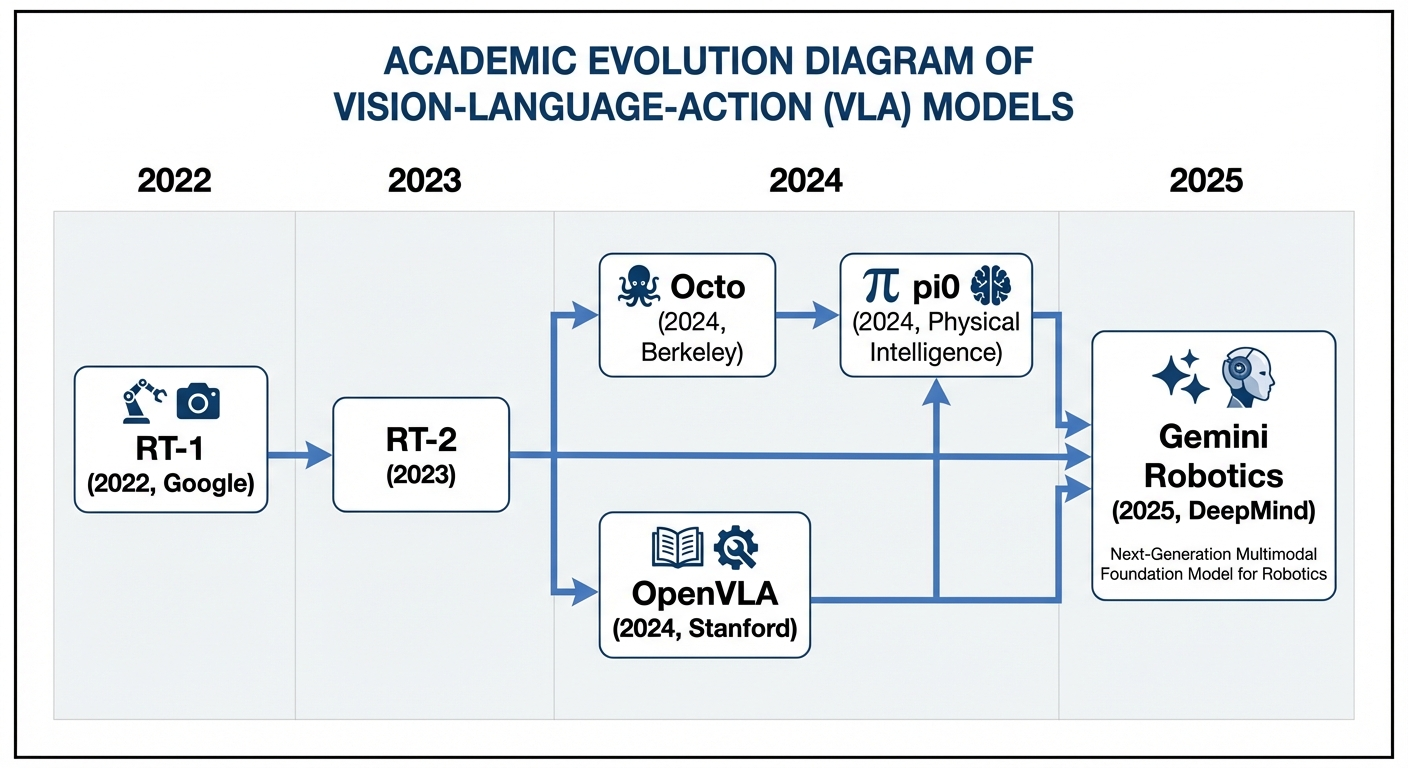
\includegraphics[width=\columnwidth]{../assets/figures/ch08/fig_8_1_vla_timeline_academic.png}
\caption{Evolution of Vision-Language-Action (VLA) models: from RT-1 (2023) through RT-2, OpenVLA, and Octo to pi0 and Gemini Robotics (2025). Each generation expanded the scope of generalist robot control through larger backbones, flow matching decoders, and cross-embodiment training.}
\label{fig:vla_timeline}
\end{figure}

\subsection{The VLA Lineage}

The VLA paradigm has evolved through several inflection points, each expanding the scope of what robot foundation models can achieve:

\textbf{RT-1}~\cite{brohan2023rt1} (Google/Everyday Robots, RSS 2023, 800+ citations) was the first large-scale Transformer trained for real-world robot control, using 130K episodes collected from 13 robots. RT-1 demonstrated that scaling up Transformer architectures and training data yields systematic improvements in manipulation success, establishing the foundation for subsequent models.

\textbf{RT-2}~\cite{brohan2023rt2} (Google DeepMind, CoRL 2023, 400+ citations) \emph{established the VLA paradigm} by fine-tuning large VLMs (PaLI-X with 55B parameters, PaLM-E with 562B parameters) on robot demonstration data. The key insight was that web-scale vision-language knowledge transfers to robotic control: RT-2 could follow novel language instructions involving objects and concepts never seen during robot training, because the underlying VLM had learned these concepts from internet data. This web-to-robot knowledge transfer fundamentally changed the field's approach to generalization.

\textbf{OpenVLA}~\cite{kim2024openvla} (Stanford/Google DeepMind, 2024, 200+ citations) democratized the paradigm with a 7B-parameter model---1/10 the size of RT-2-X---that outperformed RT-2-X while being fully open-source (weights, code, training data). OpenVLA was trained on the Open X-Embodiment dataset and demonstrated that smaller, efficiently trained models can surpass their larger predecessors.

\textbf{Octo}~\cite{octo2024} (UC Berkeley, 2024, 150+ citations) provided a generalist diffusion policy pretrained on 800K episodes from Open X-Embodiment, supporting flexible task and observation definitions with quick fine-tuning---a practical tool for researchers adapting foundation models to new hardware.

\textbf{pi0}~\cite{black2024pi0} (Physical Intelligence, 2024, 100+ citations) introduced a critical innovation: \emph{flow matching}~\cite{lipman2023flow} (ICLR 2023) for action generation. Using a PaLiGemma 3B VLM backbone with a flow matching action expert, pi0 generates actions through continuous normalizing flows rather than iterative diffusion denoising, enabling more efficient action generation. Trained on 7 robots across 68 tasks with 10{,}000+ hours of data, pi0 established the two-stage recipe---large-scale pretraining followed by task-specific post-training---that has become standard.

\textbf{Gemini Robotics}~\cite{google2025gemini} (Google DeepMind, 2025) represents the most ambitious attempt toward a ``universal robot brain,'' building VLA models on the Gemini 2.0 foundation. Gemini Robotics-ER (Embodied Reasoning) adds spatial understanding and grasp prediction to the VLA framework, enabling reasoning about physical interactions before executing them. Its application to dexterous manipulation tasks represents the frontier of VLA capability.

\subsection{Post-Deployment Improvement}

A fundamental limitation of VLA models trained via IL is failure outside the demonstration data distribution. pi0.5/RECAP~\cite{pi2025recap} addresses this through \emph{post-deployment reinforcement learning}: after initial deployment, the system collects success/failure data from real interactions and uses reinforcement learning from execution feedback (RLEF) to continuously improve the policy. This creates a deployment--learning--improvement data flywheel that progressively expands the model's competence boundary without additional human demonstrations---a critical capability for practical deployment where the full range of real-world scenarios cannot be anticipated during initial training.

\subsection{Tactile Integration in VLAs}

Integrating tactile/force information as a first-class modality in VLAs is an emerging but rapidly growing direction. Three approaches have been proposed:

\textbf{ForceVLA}~\cite{yu2025forcevla} (NeurIPS 2025) introduces FVLMoE, a 4-expert Mixture-of-Experts architecture that dynamically routes force, vision, and language inputs based on task demands. Built on a pi0-based VLA backbone, ForceVLA achieves +23.2 percentage points over force-free baselines on contact-rich tasks and maintains 90\% success under visual occlusion---conditions where vision-only models fail catastrophically. The MoE approach partially addresses the temporal resolution mismatch between vision ($\sim$30~Hz) and force/tactile (100--1{,}000~Hz) by enabling task-dependent weighting of modalities.

\textbf{Tactile-VLA}~\cite{huang2025tactilevla} takes a different approach: rather than adding new expert modules, it \emph{unlocks the physical knowledge already present} in the VLA's pretrained vision-language representations. By incorporating a hybrid position-force controller and a reasoning module that adapts strategy based on tactile feedback, Tactile-VLA demonstrates improved generalization on contact-rich tasks without the architectural overhead of MoE.

\textbf{FARM}~\cite{helmut2025farm} (ICRA 2026) integrates high-dimensional GelSight Mini tactile images directly into the Diffusion Policy framework, conditioning action denoising on tactile force profiles to enable force-aware manipulation.

The fundamental challenge remains \textbf{temporal resolution mismatch}: vision operates at $\sim$30~Hz, force/tactile sensors at 100--1{,}000~Hz, and Transformer inference introduces additional latency. No current architecture fully resolves this timing gap, making it one of the top open challenges (Section~\ref{sec:discussion}).

\subsection{Scaling and Data}

VLA performance depends strongly on data scale and diversity. \textbf{Open X-Embodiment}~\cite{oxe2024} (ICRA 2024, 300+ citations) demonstrated this dramatically: the dataset of 1M+ trajectories from 22 embodiments and 34 labs enabled RT-1-X to achieve 50\% improvement and RT-2-X to triple its performance through cross-embodiment training. \textbf{NVIDIA GR00T N1}~\cite{nvidia2025groot} provides the first open humanoid foundation model applying cross-embodiment VLA to manipulation, while GR00T N1.5 added reasoning via Cosmos Reason. NVIDIA's synthetic data pipeline---780K trajectories generated in 11 hours~\cite{nvidia2025synthetic}---demonstrates that simulation can dramatically accelerate the data flywheel when combined with domain randomization.

The systematic analysis ``What Matters in Building VLAs''~\cite{various2025whatmatters} (\emph{Nature Machine Intelligence}, 2025) examined over 600 experimental configurations across 8 VLM backbones and 4 policy architectures, finding that (1)~hierarchical or late fusion architectures outperform early fusion for generalization, and (2)~diffusion decoders consistently outperform tokenized action outputs. These findings align with ForceVLA's MoE architecture (late fusion with dynamic routing) and suggest design principles for future tactile-integrated VLAs.

\section{Human Hand Data and Embodiment Retargeting}
\label{sec:retarget}

Converting human manipulation demonstrations into robot policies requires overcoming the cross-embodiment gap---a three-dimensional challenge spanning kinematic differences (27 DoF human hand vs.\ 7--22 DoF robot), visual differences (skin, nails, and flexible tissue vs.\ metal, plastic, and rigid structure), and tactile differences ($\sim$17{,}000 human mechanoreceptors vs.\ 0--17 robot sensors). This section reviews data collection methods and solutions for each gap dimension.

\subsection{Human Hand Data Collection}

Four collection paradigms span the throughput--quality spectrum:

\textbf{Motion tracking gloves} capture joint angles and fingertip positions. A stretchable liquid-metal glove with 9 eGaIn sensors~\cite{various2024glove} (\emph{Nature Communications}, 2024) achieves 4.02~mm fingertip error with one-size-fits-all adaptation. Commercially, MANUS (designated as NVIDIA Isaac Teleop's official data glove at GTC 2026) and StretchSense (25 DoF EMF) offer higher-DoF tracking. The human hand model MANO~\cite{romero2017mano} (SIGGRAPH Asia 2017)---a statistical model learned from 1{,}000 3D scans with 778 vertices and 16 joints---serves as the foundation for virtually all retargeting work.

\textbf{Tactile gloves} capture contact forces during manipulation. STAG~\cite{sundaram2019stag} (\emph{Nature}, 548 piezoresistive sensors) provided the first large-scale tactile demonstration dataset. OSMO~\cite{yin2025osmo} (12 three-axis magnetic sensors, open-source) introduces the ``embodiment bridge'' concept---the same glove worn by human and robot eliminates the tactile domain gap entirely.

\textbf{Exoskeletons} mechanically connect to the human hand for direct motion capture with haptic feedback. DexUMI~\cite{xu2025dexumi} achieves 86\% success across Inspire and XHand with 3.2$\times$ faster data collection than teleoperation, using a wearable exoskeleton for kinematics and SAM2 inpainting for visual gap bridging. ExoStart~\cite{si2025exostart} demonstrates extreme data efficiency: from just $\sim$10 exoskeleton demonstrations, it learns dexterous policies via a MuJoCo dynamics filtering $\to$ auto-curriculum RL $\to$ ACT vision student pipeline, achieving >50\% success on 6 of 7 tasks with zero-shot real transfer. DEXOP~\cite{fang2025dexop} uses a 4-bar linkage for direct mechanical coupling between human and robot fingers, enabling 8$\times$ faster data collection with direct contact feedback (51.3\% vs.\ 42.5\% for teleoperation).

\textbf{Teleoperation} remains the standard for high-quality demonstrations. AnyTeleop~\cite{qin2023anyteleop} (RSS 2023) provides general-purpose Dex-Retarget. DexPilot~\cite{handa2020dexpilot} (NVIDIA, ICRA 2020) enables 23-DoF control from bare-hand depth images. DexCap~\cite{wang2024dexcap} (Stanford, RSS 2024) achieves 3$\times$ speedup via portable mocap with 30-minute policy learning. Internet video mining~\cite{liu2025immimic} offers unlimited scale but lacks action labels and tactile data.

\subsection{Kinematic Retargeting}

The kinematic gap---mapping 27 human DoF to 7--22 robot DoF---is the most studied dimension. Three approaches reflect increasing sophistication:

\textbf{Joint-level mapping} (AnyTeleop's Dex-Retarget~\cite{qin2023anyteleop}) directly maps human keypoints to robot joint positions. While general-purpose, naive mapping often produces physically infeasible robot poses due to kinematic differences in joint ranges, coupling, and workspace.

\textbf{Data interpolation} (ImMimic~\cite{liu2025immimic}) takes a data-centric approach: large-scale human trajectories (diverse but potentially infeasible for the robot) are interpolated with a few teleoperation trajectories (feasible but limited in diversity). This augmentation preserves the diversity of human data while maintaining physical feasibility.

\textbf{Intent-level transfer} (DexH2R~\cite{li2024dexh2r}) extracts the task-level \emph{intent} of human demonstrations---what the manipulation is trying to achieve---and reproduces that intent within the robot's kinematic constraints, rather than attempting joint-level correspondence.

\subsection{Visual Gap}

Visual policies trained on robot data fail when the input contains human hands instead of robot end-effectors. Two approaches bridge this gap:

\textbf{DexUMI}~\cite{xu2025dexumi} uses SAM2 segmentation and inpainting to \emph{erase the human hand from camera images} and replace it with a high-fidelity rendering of the robot hand, making visual policies embodiment-agnostic. \textbf{RoboPaint}~\cite{various2026robopaint} uses 3D Gaussian Splatting (3DGS) to reconstruct real scenes in simulation with photorealistic fidelity, reducing the visual sim-to-real gap in Real-Sim-Real loops.

\subsection{Tactile Gap}

The tactile gap---$\sim$17{,}000 human mechanoreceptors distributed across the entire hand versus 0--17 discrete sensors on a robot---is the least studied and hardest to resolve. Two fundamentally different approaches have been proposed:

\textbf{UniTacHand}~\cite{zhang2025unitachand} takes a \emph{software} approach: human glove tactile data and robot hand tactile data are both projected onto MANO UV maps, creating a shared 2D representation space. Contrastive learning with reconstruction and adversarial losses aligns the latent representations, enabling zero-shot or one-shot human-to-robot tactile policy transfer. This is the \emph{only} paper that systematically addresses tactile cross-embodiment transfer. Limitation: requires MANO-compatible hand geometry.

\textbf{OSMO}~\cite{yin2025osmo} takes a \emph{hardware} approach: by placing identical 12-sensor three-axis magnetic gloves on both human and robot, the tactile domain gap is \emph{physically eliminated}---same sensors produce identical signals regardless of embodiment. A robot policy trained exclusively on human OSMO data, without any robot data, successfully executes contact-rich manipulation tasks. Limitation: requires identical sensor hardware on both embodiments.

\textbf{Open challenge}: No general methodology exists for tactile cross-embodiment transfer. UniTacHand requires MANO-compatible hands; OSMO requires identical hardware; DEXOP~\cite{fang2025dexop} depends on mechanical coupling form factor. Extending sensor-agnostic representation approaches (AnyTouch~\cite{feng2025anytouch}, Sensor-Invariant~\cite{various2025sensorinvariant}) to cross-embodiment settings, and developing universal tactile UV maps applicable beyond MANO, represent critical future directions.

\section{Integrated Systems and Applications}
\label{sec:systems}

The preceding sections reviewed individual components---sensors, hands, data, learning methods, VLA models, and retargeting. This section examines how these components integrate into unified systems, the open-source ecosystem accelerating this integration, and the current state of industrial deployment.

\subsection{Multi-Modal Fusion Architectures}

Combining tactile with visual and/or language information requires architectural choices that significantly impact performance. Four fusion paradigms have emerged:

\textbf{Early fusion} concatenates raw or low-level features from different modalities before joint processing. 3D-ViTac~\cite{huang2024vitac} (CoRL 2024) exemplifies this approach, fusing 3~mm$^2$-resolution dense tactile sensor data with visual observations into a unified 3D representation processed by Diffusion Policy. The result---85--90\% success on bimanual dexterous tasks versus 45--50\% with vision only---demonstrates the magnitude of improvement tactile integration provides, though early fusion risks cross-modal interference when sensor characteristics differ significantly.

\textbf{Late fusion} processes each modality through independent stream networks, combining only at the decision level. NeuralFeels~\cite{suresh2024neuralfeels} (\emph{Science Robotics}, 2024) uses neural fields to independently process visual and tactile inputs for visuotactile in-hand SLAM, estimating object pose and shape simultaneously during manipulation---a task impossible with either modality alone due to finger occlusion. The late fusion approach preserves modality-specific processing but limits cross-modal interaction during feature extraction.

\textbf{Mixture of Experts (MoE)} dynamically routes inputs through specialized expert networks based on task demands. ForceVLA~\cite{yu2025forcevla} (NeurIPS 2025) implements this with FVLMoE: four expert modules process force, vision, and language combinations with learned gating, achieving task-dependent optimal weighting. This architecture naturally handles the temporal resolution mismatch (vision at 30~Hz vs.\ force at 1{,}000~Hz) through adaptive routing.

\textbf{Attention-based fusion} uses Transformer cross-attention mechanisms to learn inter-modal relationships. Most VLA architectures (RT-2, pi0, Gemini Robotics) implicitly implement attention-based fusion for vision-language, with tactile tokens increasingly being added to the attention mechanism.

Robot Synesthesia~\cite{yuan2024synesthesia} (ICRA 2024) demonstrated an innovative approach: converting tactile signals into point clouds processable by PointNet alongside visual point clouds, enabling visuotactile in-hand manipulation that generalizes to novel objects via teacher-student RL.

\subsection{End-to-End Systems}

Several systems demonstrate the value of full-pipeline integration:

\textbf{Mobile ALOHA}~\cite{fu2024mobilealoha} (Stanford, 200+ citations) combines a mobile base with bimanual ALOHA arms and ACT-based policy learning into the most influential end-to-end research platform. Its impact stems from the combination of low cost (sub-\$20K), open-source design, and demonstrated capability across diverse household tasks.

\textbf{PP-Tac}~\cite{lin2025pptac} (RSS 2025) integrates R-Tac tactile sensor, slip detection CNN, online force controller, and Diffusion Policy into a unified pipeline for 87.5\% thin-object grasping---demonstrating that practical, problem-specific integration of sensing, perception, control, and learning yields immediate practical value.

\textbf{TacEx}~\cite{various2024tacex} integrates GelSight simulation into NVIDIA Isaac Sim, providing a complete research workflow---sensor simulation, policy learning, and sim-to-real transfer---in a single platform, reducing the engineering burden of multi-tool research pipelines.

The \textbf{temporal integration} of intelligent mechanisms (Section~\ref{sec:mechanisms})---underactuation for shape adaptation, VSA for grasp locking, active surfaces for in-grasp manipulation---represents a hardware-level end-to-end system designed for factory scenarios involving thin objects, multiple objects, and repositioning.

\subsection{Open-Source Ecosystem}

The democratization of dexterous manipulation research is driven by an open-source ecosystem spanning three layers:

\textbf{Hardware}: LEAP Hand~\cite{shaw2023leap} (\$2K), ORCA~\cite{christoph2025orca} (17 DoF + tactile), ISyHand~\cite{richardson2025isyhand} (\$1.3K + articulated palm), OSMO glove~\cite{yin2025osmo} (tactile bridge), DOGlove~\cite{zhang2025doglove} (\$600 haptic feedback). Before 2023, dexterous manipulation research required \$16K--100K in hardware; now it starts at \$2K.

\textbf{Software}: OpenVLA~\cite{kim2024openvla} (7B open VLA), Octo~\cite{octo2024} (generalist policy), Diffusion Policy~\cite{chi2023diffusion}, ACT/ALOHA~\cite{zhao2023aloha}. These open-weight models enable researchers to fine-tune state-of-the-art policies without training from scratch.

\textbf{Data}: Open X-Embodiment~\cite{oxe2024} (1M+ trajectories, 22 embodiments), Touch-and-Go~\cite{yang2022touchandgo} (3M+ contacts), Touch100k~\cite{yang2024touch100k}, VTDexManip~\cite{liu2025vtdexmanip} (10 tasks, 182 objects). Shared data eliminates the coldstart problem for new research groups.

This triple-layer ecosystem has reduced the cost, time, and expertise required to enter dexterous manipulation research by an order of magnitude, accelerating the pace of discovery.

\subsection{Industrial Deployment and Market Outlook}

Current humanoid robot factory deployments have achieved commercial validation at the logistics level:

\begin{itemize}
    \item \textbf{Figure AI} at BMW Spartanburg: 10-month deployment, 90K components moved, contributing to 30K BMW X3 production~\cite{figureai2025}.
    \item \textbf{Agility Robotics (Digit)} at Amazon/GXO: 100K+ totes recycled in fulfillment centers.
    \item \textbf{Boston Dynamics (Electric Atlas)} at Hyundai: Factory fleet deployment in progress.
    \item \textbf{Apptronik (Apollo)} at Mercedes Berlin: Intra-logistics pilot.
    \item \textbf{Sanctuary AI (Phoenix)} at Magna: Automotive parts sorting pilot with 5~mN tactile sensitivity---the most advanced tactile integration among commercial humanoids.
\end{itemize}

The critical observation: \emph{all current deployments remain at the logistics (pick-move-place) level. Dexterous assembly has not yet reached production floors}~\cite{billard2019trends}. The gap between logistics-level deployment and manufacturing-grade dexterous manipulation---where tactile feedback is essential for force control, slip detection, and quality assurance---defines the central challenge for the next 3--5 years. The humanoid market is projected to grow from \$2.9B (2025) to \$15.3B (2030) at 39.2\% CAGR, driven by automotive beachhead deployments, with Sanctuary AI's tactile integration and Figure AI's VLA-based control representing the leading approaches to bridging the logistics-to-dexterity gap.

\section{Open Challenges and Future Directions}
\label{sec:discussion}

This section synthesizes the findings of the preceding sections into a systematic analysis of the field's most pressing challenges and promising future directions. We identify the top 10 open challenges based on frequency analysis across 146 papers, organize future research directions into five groups, and propose the mechanism--tactile--learning triangle as a unifying research agenda.

\subsection{Top 10 Open Challenges}

Analysis of 146 papers published between 2020 and 2026 reveals 10 recurring limitations, organized by frequency of mention:

\begin{enumerate}
    \item \textbf{Sim-to-Real Gap} (mentioned in 20+ papers): The tactile sim-to-real gap is fundamentally harder than the visual sim-to-real gap due to gel deformation physics, multi-physics coupling (optical + mechanical + thermal), and contact model fidelity limitations~\cite{handa2023dextreme,openai2020dactyl,si2024difftactile}. While domain randomization~\cite{handa2023dextreme} and simplified binary models~\cite{yin2024tactile} partially mitigate this gap, no approach has achieved the level of tactile simulation fidelity that Omniverse Replicator provides for visual rendering. DiffTactile~\cite{si2024difftactile} addresses fidelity through differentiable simulation but at computational costs that preclude the massive parallelism (thousands of environments) that GPU-accelerated RL requires.

    \item \textbf{Novel Object Generalization} (15+ papers): Policies trained on specific objects fail when encountering unseen shapes, sizes, and---critically---material properties. Vision cannot capture friction, compliance, or surface texture with the fidelity needed for reliable manipulation. VLA models show improved semantic generalization (recognizing novel objects from language descriptions) but still struggle with \emph{physical} generalization (adapting grip force and manipulation strategy to unfamiliar material properties)~\cite{kim2024openvla,black2024pi0,google2025gemini}. This gap motivates tactile integration as a pathway to material-aware manipulation.

    \item \textbf{Sensor Durability} (12+ papers): Current tactile sensors cannot withstand long-term industrial use. Vision-based sensors degrade with gel wear, light source degradation, dust infiltration, and cleaning difficulty. The F-TAC Hand's 17 sensors create 17 potential failure points~\cite{zhao2025ftac}. AnySkin's 12-second replacement~\cite{bhirangi2024anyskin} offers a practical mitigation but not a fundamental solution. No sensor has published MTBF (mean time between failures) data suitable for industrial certification.

    \item \textbf{Data Scarcity} (12+ papers): High-quality demonstration data remains the primary bottleneck. Teleoperation yields $\sim$10 demos/hr~\cite{wang2024dexcap}; force and tactile data are particularly expensive to collect because they require physical contact~\cite{chen2025dexforce}. NVIDIA's synthetic data pipeline (780K trajectories in 11 hours)~\cite{nvidia2025synthetic} addresses scale for visual data, but extending this to high-fidelity tactile data remains limited by the tactile sim-to-real gap (Challenge \#1).

    \item \textbf{Hardware Cost and Fragility} (10+ papers): Despite the open-source revolution (Shadow \$100K $\to$ LEAP \$2K), research-grade dexterous hands remain fragile. Multi-fingered hands amplify breakage risk during exploration-heavy RL training. No published MTBF data exists for any research hand, making industrial certification impossible~\cite{shaw2023leap}.

    \item \textbf{Cross-Embodiment Transfer} (10+ papers): Policies trained on one hand morphology do not transfer to different hands. The tactile dimension is the least resolved: UniTacHand~\cite{zhang2025unitachand} is the \emph{only} paper systematically addressing tactile cross-embodiment transfer, and its MANO UV map approach is limited to MANO-compatible hand geometries. OSMO~\cite{yin2025osmo} eliminates the gap through identical hardware but cannot generalize across different sensor types.

    \item \textbf{Multi-Modal Fusion Timing} (8+ papers): Vision operates at $\sim$30~Hz while force/tactile sensors run at 100--1{,}000~Hz, creating a fundamental temporal alignment challenge~\cite{yu2025forcevla,suresh2024neuralfeels}. Transformer-based architectures introduce additional inference latency. ForceVLA's MoE approach~\cite{yu2025forcevla} partially addresses this through dynamic routing but does not fully resolve the timing mismatch for real-time control.

    \item \textbf{Safety in Human Proximity} (7+ papers): ISO/TS 15066 compliance---the standard for collaborative robot safety---has not been demonstrated by any current dexterous manipulation system~\cite{billard2019trends}. High-power actuators needed for dexterous manipulation conflict with the force/power limits required for human safety.

    \item \textbf{Long-Horizon Tasks} (7+ papers): Error compounding in multi-step tasks beyond 5--30 seconds remains a critical limitation of both IL and VLA approaches~\cite{black2024pi0,google2025gemini}. Current systems lack robust error recovery mechanisms that would enable autonomous recovery from intermediate failures during extended manipulation sequences.

    \item \textbf{Evaluation Standardization} (6+ papers): No established benchmark exists for tactile sensor performance comparison. Vision has ImageNet and COCO; tactile has nothing comparable. The RGMC competition~\cite{yu2025rgmc} provides manipulation evaluation but lacks tactile-specific metrics. Albini et al.'s data structure taxonomy~\cite{albini2025representing} may serve as a foundation for standardization.
\end{enumerate}

\subsection{Future Research Directions}

We organize future directions into five interconnected groups:

\textbf{A. Sensing and Perception.} Tactile foundation models need 10$\times$+ data expansion beyond Sparsh's 460K images~\cite{higuera2024sparsh} to match the robustness of visual foundation models. Neuromorphic event-driven sensors~\cite{gao2025nreskin} promise orders-of-magnitude improvements in energy efficiency and temporal resolution. Self-healing and self-calibrating sensor materials would address the durability challenge at a fundamental level. Whole-hand dense tactile coverage (F-TAC Hand direction~\cite{zhao2025ftac}) should become standard rather than exceptional. Sensor-agnostic representations (AnyTouch~\cite{feng2025anytouch}) need extension to cross-embodiment settings.

\textbf{B. Learning and Control.} VLA models should integrate tactile as a first-class modality alongside vision and language~\cite{yu2025forcevla,huang2025tactilevla}. Post-deployment RL (pi0.5/RECAP paradigm~\cite{pi2025recap}) should extend to tactile-conditioned continuous improvement. One-/zero-shot learning from internet video~\cite{liu2025immimic} could bypass the teleoperation bottleneck if combined with tactile data augmentation. Hierarchical VLA architectures with error recovery mechanisms are needed for long-horizon dexterous tasks. World models incorporating tactile feedback would enable model-based planning for contact-rich scenarios.

\textbf{C. Hardware and Design.} Sub-\$1K dexterous hands combining LEAP-level cost with F-TAC-level tactile coverage are technically feasible and would further democratize the field. Modular, replaceable sensor skins (AnySkin direction~\cite{bhirangi2024anyskin}) should reduce maintenance to minutes rather than hours. Variable stiffness actuators co-optimized for safety and dexterity would address the safety challenge. Standardized hand-sensor interfaces (Digit Plexus direction) would enable mix-and-match hardware ecosystems.

\textbf{D. Data and Simulation.} Tactile simulation fidelity must improve to close the tactile sim-to-real gap (DiffTactile~\cite{si2024difftactile}, TacEx~\cite{various2024tacex}). NVIDIA's 780K-trajectory approach~\cite{nvidia2025synthetic} should be extended to include high-fidelity tactile rendering at GPU-accelerated speeds. Shared tactile datasets need to scale from 3M contacts (Touch-and-Go) to 100M+ for robust foundation model training. Cross-embodiment data reuse frameworks (extending OXE~\cite{oxe2024} to include hand-specific tactile data) would multiplicatively increase effective dataset size.

\textbf{E. Deployment and Application.} Functional safety certification for human-proximity dexterous manipulation is a prerequisite for production deployment. Tactile-based quality inspection---detecting defects invisible to cameras through touch---represents a high-value industrial application. Deformable material handling (textiles, cables, food) at production speeds, and multi-robot collaborative manipulation (building on Helix dual-robot demonstrations), are near-term deployment targets.

\begin{figure}[t]
\centering
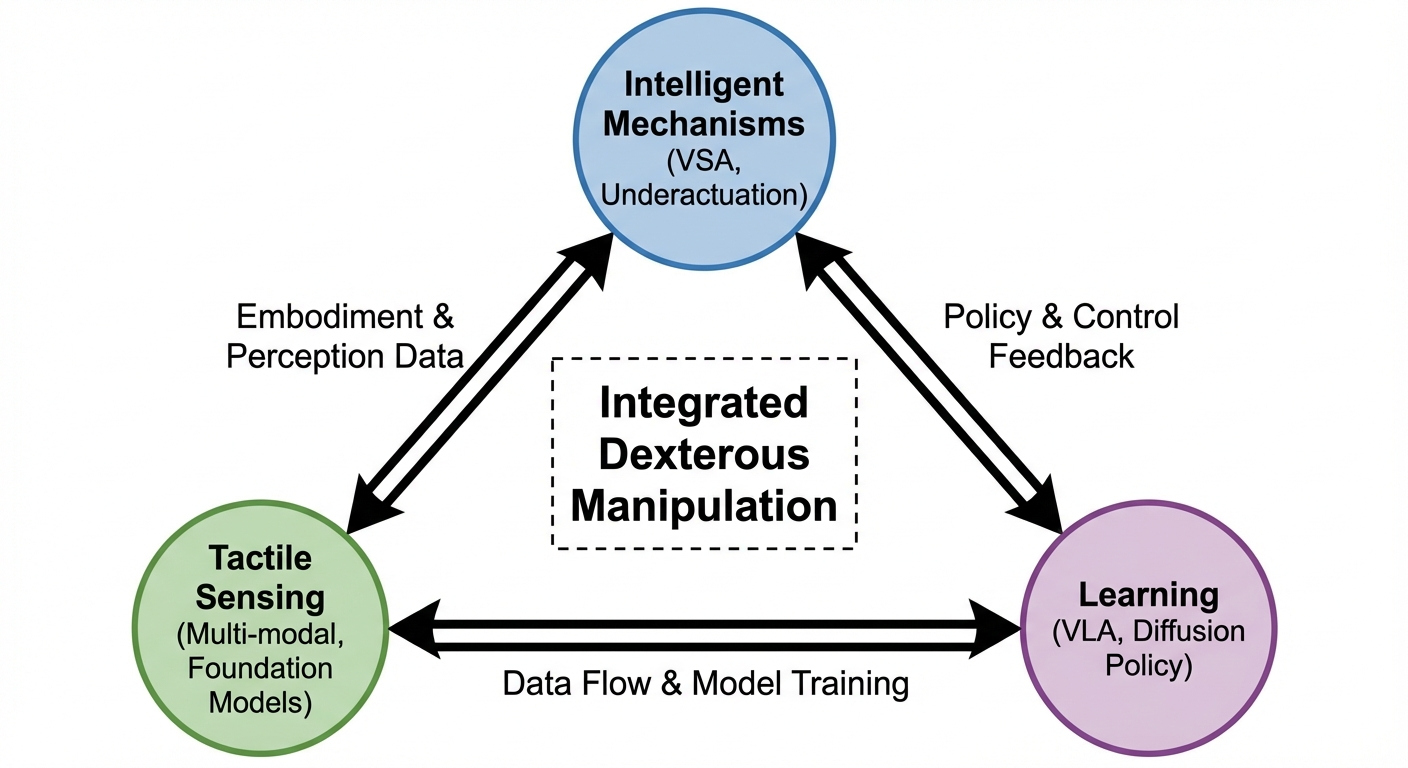
\includegraphics[width=\columnwidth]{../assets/figures/ch13/fig_13_4_triangle_integration_academic.png}
\caption{The proposed mechanism--tactile--learning triangle: intelligent mechanisms physically guarantee continuous contact, tactile sensors recognize the contact state, and learned policies exploit this information. The synergy among the three axes reduces the burden on each individual component and improves overall system robustness.}
\label{fig:triangle}
\end{figure}

\subsection{The Mechanism--Tactile--Learning Triangle}

We propose a unifying research direction that synthesizes the central insights of this survey:

\begin{itemize}
    \item \textbf{Mechanism axis} (Physical Intelligence): Intelligent mechanisms---underactuation, VSA, active surfaces, and their temporal integration---\emph{physically guarantee} continuous contact during manipulation (Section~\ref{sec:hands}). This improves state stability, simplifies the control problem, and reduces the frequency of destabilizing contact state transitions.

    \item \textbf{Tactile axis} (Sensing): Tactile sensors recognize the contact state during mechanism-induced continuous contact (Section~\ref{sec:sensors}), providing precise force measurement, slip detection, and material property estimation that enable closed-loop force control.

    \item \textbf{Learning axis} (Policy): VLA/Diffusion policies exploit the stable, information-rich tactile feedback from continuous contact states (Sections~\ref{sec:learning}--\ref{sec:vla}), achieving higher sample efficiency and better generalization than policies operating under the uncertainty of intermittent contact.
\end{itemize}

The key proposition is that \emph{when mechanism physically guarantees continuous contact, tactile recognizes the contact state, and learning exploits this information, the burden on each individual axis is reduced and the overall system robustness improves superlinearly}. The mechanism axis reduces the sensing challenge (stable contact $\to$ cleaner signals); the tactile axis reduces the learning challenge (rich feedback $\to$ fewer samples needed); and the learning axis enables the mechanism to be deployed in diverse, unstructured scenarios that pure mechanism design cannot anticipate.

This triangle connects the ``physical intelligence'' explored in Section~\ref{sec:mechanisms} with the ``software intelligence'' of Sections~\ref{sec:learning}--\ref{sec:vla}, offering a concrete path from current logistics-level industrial deployment to the manufacturing-grade dexterous manipulation that the field ultimately seeks. The key research question is: \emph{how should mechanism design, sensor placement, and policy architecture be jointly optimized to maximize the synergy among these three axes?}

\section{Conclusion}
\label{sec:conclusion}

This survey has provided a comprehensive review of tactile sensing for dexterous robot manipulation, spanning sensor technologies, hand design, data representation, learning methods, VLA models, and embodiment retargeting. Our analysis of 146 papers (2020--2026) reveals three converging trends that are driving the field at unprecedented pace: (1) cost reduction of vision-based sensors (BioTac \$10K $\to$ DIGIT \$350 $\to$ ReSkin \$6), (2) democratization of open-source hands (Shadow \$100K $\to$ LEAP \$2K), and (3) emergence of VLA foundation models (RT-2 $\to$ pi0 $\to$ Gemini Robotics) with nascent tactile integration (ForceVLA, Tactile-VLA).

We identified the top 10 open challenges, led by the tactile sim-to-real gap and the absence of general solutions for cross-embodiment tactile transfer. Current industrial deployments remain at the logistics level; dexterous assembly has not yet reached production floors. To bridge this gap, we proposed the mechanism--tactile--learning triangle, which combines physical intelligence (underactuation, VSA, active surfaces) with tactile perception and learned policies to reduce the burden on each individual axis.

As of 2026, tactile sensing is transitioning from optional to standard in humanoid robotics. Sanctuary AI has integrated 5~mN sensitivity into a commercial platform, NVIDIA generates 780K synthetic trajectories in 11 hours, and pi0.5/RECAP demonstrates continuous post-deployment improvement. The question is no longer \emph{whether} robots need touch, but \emph{how quickly} the field can deliver manufacturing-grade dexterous manipulation. We hope this survey accelerates that transition.


\section*{Acknowledgment}
This work was conducted with the assistance of artificial intelligence tools, including Claude (Anthropic) for literature survey, content generation, and manuscript preparation, and Gemini (Google) for figure generation. The authors take full responsibility for the accuracy and integrity of the content presented in this paper.

\bibliographystyle{IEEEtran}
\bibliography{references}

\end{document}
